\section{Introduction} \label{sec:introduction}
    \IEEEPARstart{R}{espiratory} motion correction is beneficial in \gls{PET}; respiratory motion reduces image resolution by introducing blurring and mis-alignment artefacts~\cite{Nehmeh2008a}. Methods of motion correction including gated reconstruction bin the acquisition based on a surrogate signal. This surrogate signal is a respiratory trace which reflects the position of the patient in the respiratory cycle over time~\cite{Kesner2010AMethods, Kesner2013GatingPET}. Methods to determine the surrogate signal include those which use an external device, for instance, the \gls{RPM}~\cite{Bettinardi2013Motion-trackingPET/CT}. A disadvantage of such methods are that they require the use of additional equipment and a change to clinical practise. Thus, data driven methods to extract the surrogate signal have become an alternative for static PET data. %XXX Need to give a brief overview of data-driven methods here with citations. XXX
    
    \gls{PCA} has been successfully used to extract a respiratory signal from \gls{PET} acquisition data \cite{Thielemans2011, Bertolli2018Data-DrivenTomography}. Such methods rely on the fact that, in static \gls{PET}, the main cause of (non-stochastic) change in the data is motion. A respiratory signal was therefore extracted from one of the first principal components. Evaluations have previously been performed on static \gls{18F-FDG} PET data to compare the results of the \gls{PCA} to both \gls{RPM} and \gls{MR} navigator based surrogate signals. When compared to both external methods \gls{PCA} was shown to be relatively robust, specifically showing a correlation of $0.89$ over nine patients when compared to the \gls{MR} navigator based surrogate signals~\cite{Thielemans2013ComparisonData, Manber2015PracticalPET/MR.}.
    
    % XXX, SAM, COD, Kessner, etc
    
    However, current data driven methods are adversely affected by the radiotracer kinetics of a dynamic acquisition; where the tracer is injected after the beginning of the scan. As an example, methods that use dimensionality reduction (such as \gls{PCA}) are hampered by the fact that at the start of the scan, rapid redistribution of the radiotracer causes more variance in the data than the respiratory motion.
    
    % XXX need to describe any attempts at this in the literature XXX
    
    Previously, work was performed to extend the \gls{SAM} method to be robust to radiotracer kinetics, this work proposed the use of \gls{STFT} to generate masks for \gls{SAM} (rather than a static mask for all time points), this was called \gls{KRG}~\cite{Schleyer2014}. \gls{STFT} operates by splitting the data into windows and doing a \gls{FFT} on them independently, this could be approximated by windowing the data first and then performing \gls{SAM}.
    
    The aim of the current work is to propose several adaptions of the \gls{PCA} method through which it can be used with dynamic data and compare their performance with a method based on \gls{KRG}. The methods explored in this work include the use of a moving window, re-use of the \glss{PC} from a later time point to estimate the surrogate signal from earlier time points and the automatic selection and combination of multiple \glss{PC}.

% \vspace{-0.3cm}
    
\section{Methods} \label{sec:methods}
    \subsection{Data Acquisition} \label{sec:data_acquisition}
        Data used was acquired from a research study with patients suffering from idiopathic pulmonary fibrosis. $21$ dynamic \gls{18F-FDG} acquisitions, with a \gls{FOV} covering the upper lung and heart, were acquired on a \gls{GE} Discovery $710$ in list-mode. Data used in this study was from the first \SI{20}{\minute} with the acquisition starting roughly \SI{20}{\second} before injection of the radiotracer. Surrogate signals were acquired in parallel using an \gls{RPM}~\cite{Oh2019OptimalTreatment, Emond2020EffectReconstruction}.
    
    % \vspace{-0.3cm}
        
    \subsection{Data Preparation} \label{sec:data_preparation}
        Data were unlisted into low spatial resolution sinograms, each with time frame duration of \SI{500}{\milli\second}, using the \gls{GE} PetToolbox following~\cite{Bertolli2017DataData} resulting in sinograms with dimensions $95 x 16 x 47 x 11$ (radial positions $x$ angles $x$ transaxial plane $x$ \gls{TOF}). Usually when used to extract respiratory variation the sampling rate of the \gls{PET} sinograms is chosen as \SI{2}{\hertz} so as to attempt to mitigate cardiac motion by averaging most of it in each frame while still allowing for respiratory motion between frames~\cite{Bertolli2018Data-DrivenTomography}.
        
        Data was pre-processed by first applying a Freeman-Tukey transformation~\cite{Freeman1950TransformationsRoot} before then applying a Yeo-Johnson power transformation~\cite{Yeo2000ASymmetry}, this is in order to attempt to transform the Poisson distributed data to be more Gaussian-like. The Freeman-Tukey transformation was applied before the Yeo-Johnson power transformation as it was found that the preapplication of the Freeman-Tukey transformation lead to the Yeo-Johnson power transformation giving more robust results. Furthermore, it was also found that adding the Yeo-Johnson power transformation gave better results than the Freeman-Tukey transformation alone.
        
        The Freeman-Tukey transformation is defined as:
        
        \begin{equation} \label{eq:freeman_tukey}
            S_g := \sqrt{S_p + 1} + \sqrt{S_p}
        \end{equation}
        
        \noindent where in~\Fref{eq:freeman_tukey} $S_g$ is the resultant, approximately Gaussian distributed, sinogram and $S_p$ is the original Poisson distributed sinogram $S_p$~\cite{Freeman1950TransformationsRoot}.
        
        The Yeo-Johnson power transformation is defined as:
        
        \begin{equation} \label{eq:yeo_johnson}
            S_g := \begin{cases}
                        ((S_p + 1)^\lambda - 1) / \lambda                   & \quad \text{if } \lambda \neq 0 \text{, } S_p \geq 0 \\
                        \log(S_p + 1)                                       & \quad \text{if } \lambda = 0 \text{, } S_p \geq 0    \\
                        -[(-S_p + 1)^{(2 - \lambda)} - 1)] / (2 - \lambda)  & \quad \text{if } \lambda \neq 2 \text{, } S_p < 0    \\
                        -\log(-S_p + 1)                                     & \quad \text{if } \lambda = 2 \text{, } S_p < 0
                    \end{cases}
        \end{equation}
        
        \noindent where in~\Fref{eq:yeo_johnson} $S_g$ is the resultant, approximately Gaussian distributed, sinogram. The $\lambda$ parameter is determined by minimising the Kullback-Leibler distance between normal distributions and the transformed distribution~\cite{Yeo2000ASymmetry}. In the current implementation, a single $\lambda$ is determined from all of the data, although it would be feasible to find different $\lambda$ values for every element in the sinogram.
        
        The resultant sinograms are further spatially downsampled. This is for a number of reasons including; that the noise present in the full data would obscure the motion. It has been found through experimentation that Gaussian smoothing can improve results, especially in the case of the \gls{SAM} methods~\cite{Thielemans2013ComparisonData}. Further downsampling can be performed post-smoothing to reduce memory usage, in this case linear interpolation has been found to be satisfactory and additionally is less computationally expensive to calculate than some methods. Values for both the Gaussian smoothing and spatial downsampling were determined using a grid search.
        
        Additionally, it has been found that the introduction of a mask to further aid in the reduction of noise is beneficial \cite{Thielemans2011}. Both types of method can be used with a mask. The mask itself is defined as being true for any value in the sinogram above a predetermined threshold, values not in the mask are removed prior to further execution. Note that a mask can also be used to eliminate parts of the data potentially affected by non-respiratory movement~\cite{Bertolli2018Data-DrivenTomography}, but this has not been implemented in the current method.
    
    % \vspace{-0.3cm}
        
    \subsection{Surrogate Signal Extraction} \label{sec:surrogate_signal_extraction}
        \begin{figure}
            \centering
        
            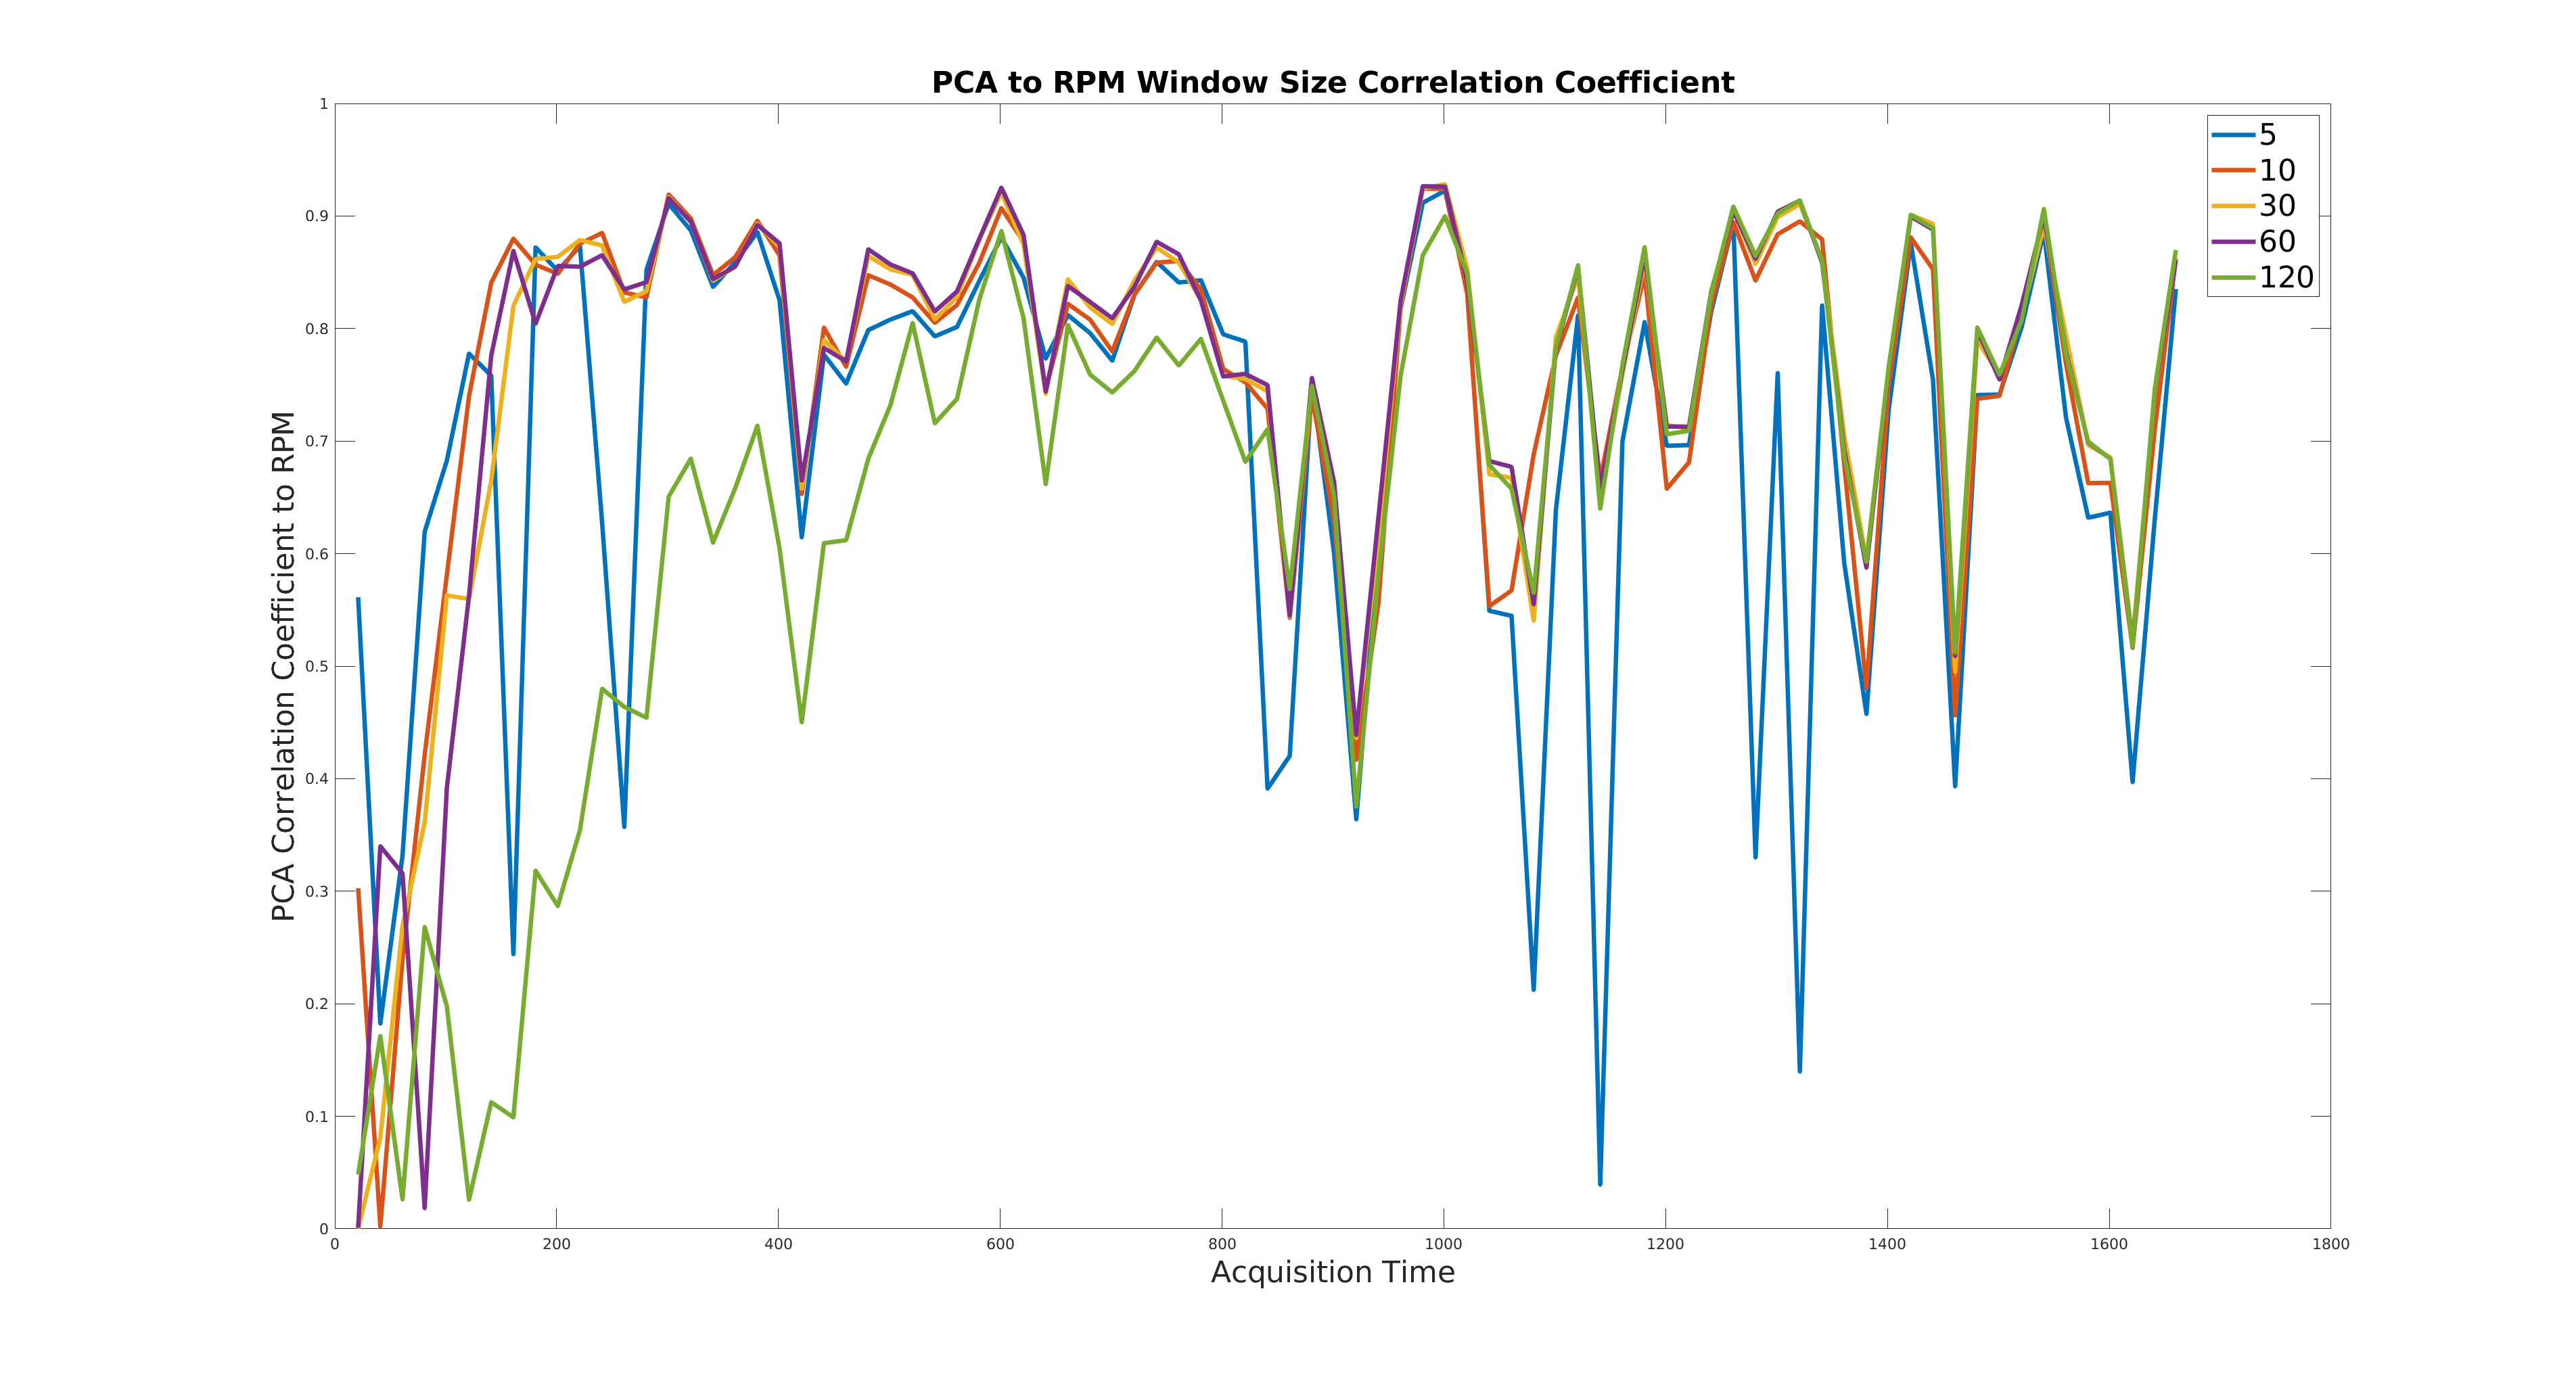
\includegraphics[width=1.0\linewidth]{figures/pca_window_correlation_coefficient.png}
        
            \captionsetup{singlelinecheck=false, justification=centering}
            \caption{A plot showing for the Moving Window \gls{PCA} method, using different fixed window sizes, its output compared to the \gls{RPM} (taken for the first acquisition of patient one).}
            \label{fig:pca_window_correlation_coefficient}
        \end{figure}
        
        \begin{figure}
            \centering
        
            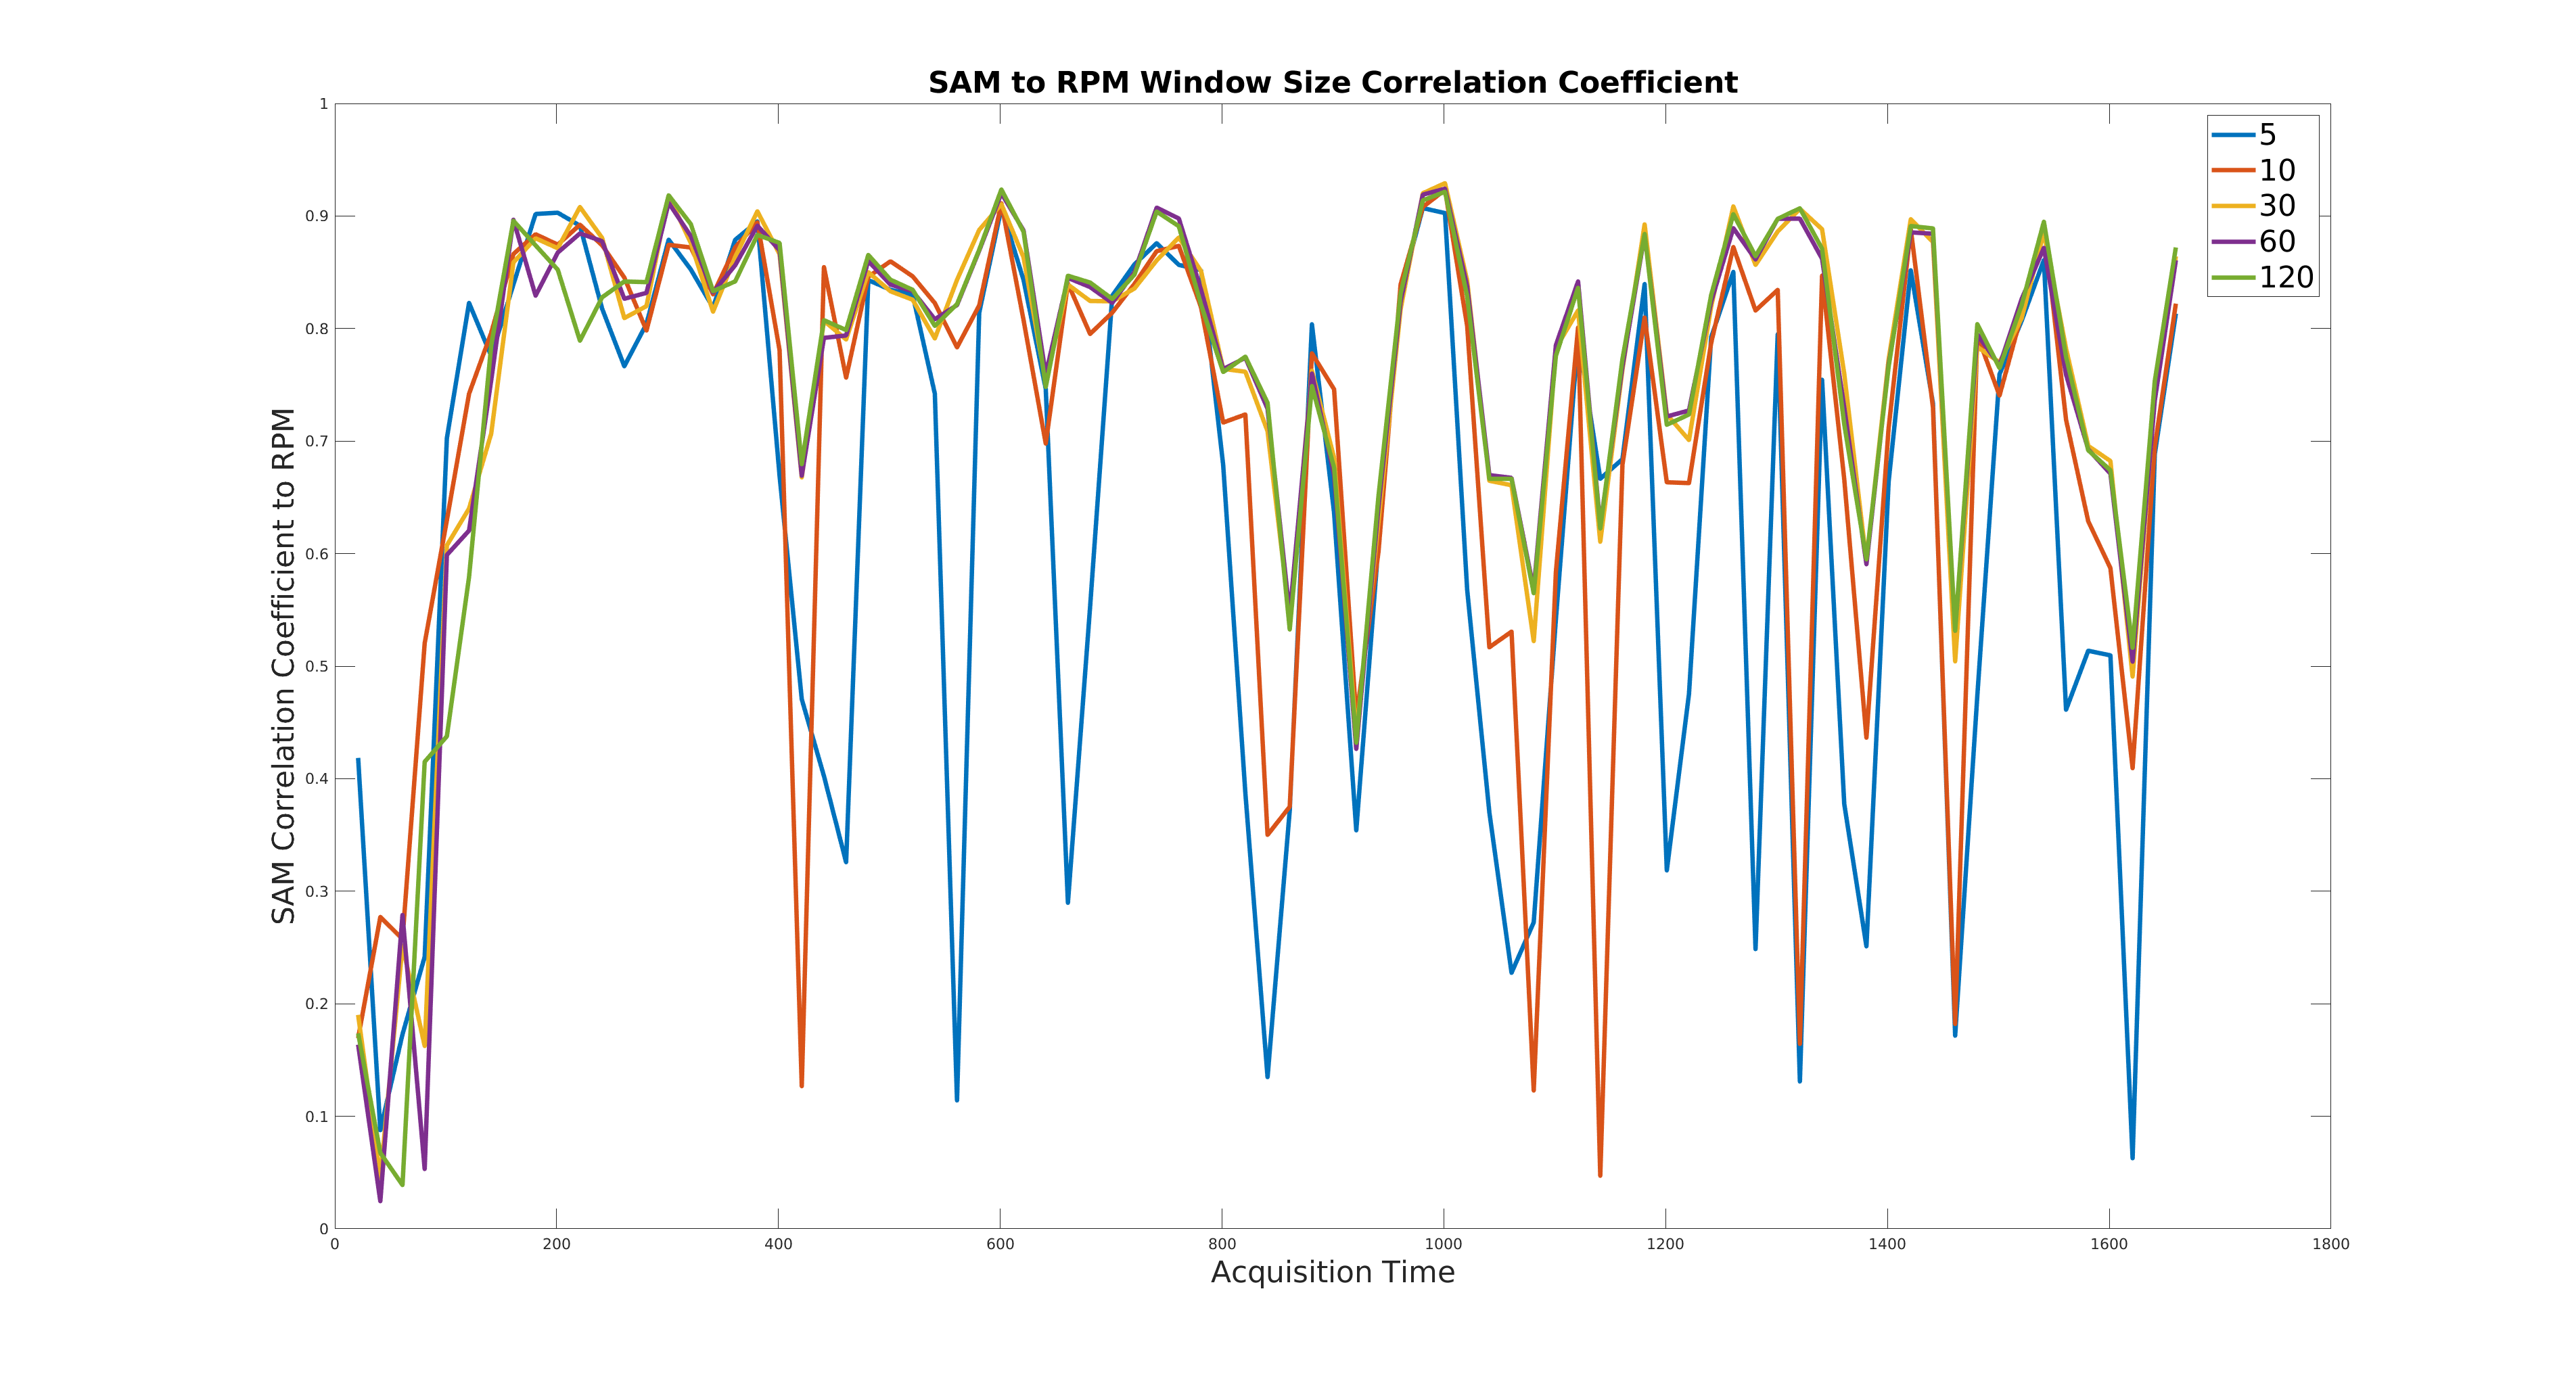
\includegraphics[width=1.0\linewidth]{figures/sam_window_correlation_coefficient.png}
        
            \captionsetup{singlelinecheck=false, justification=centering}
            \caption{A plot showing for the Moving Window \gls{SAM} method, using different fixed window sizes, its output compared to the \gls{RPM} (taken for the first acquisition of patient one).}
            \label{fig:sam_window_correlation_coefficient}
        \end{figure}
        
        Here we describe three methods that are either simple modifications of the static methods or based on \gls{KRG}. These methods can be used with \gls{SAM} but for simplicity we will refer specifically to \gls{PCA}.
        
        \subsubsection{Static \gls{PCA}} \label{sec:static_pca}
            \begin{algorithm}
                \caption{Get score}
                \KwData{\glss{PC}, $kineticFrequencyWindow$, $respiratoryFrequencyWindow$, $noiseFrequencyWindow$}
                \KwResult{$respiratoryScore$}
                \;
                $PSD$ := \gls{FFT} on current \gls{PC}\;
                \;
                $kineticContribution$ := max value of $PSD$ within $kineticFrequencyWindow$\;
                $respiratoryContribution$ := max value of $PSD$  within $respiratoryFrequencyWindow$\;
                $noiseContribution$ := max value of $PSD$ within $noiseFrequencyWindow$\;
                \;
                $respiratoryKineticRatio$ := $respiratoryContribution$ / $kineticContribution$\;
                $respiratoryNoiseRatio$ := $respiratoryContribution$ / $noiseContribution$\;
                \;
                $respiratoryScore$ := $respiratoryKineticRatio$ * $respiratoryNoiseRatio$\;
            \end{algorithm} \label{eq:get_score_pseudo_code}
            
            Here, \gls{PCA} is applied to the entire data set in one go as it would be if the data were from a static acquisition.
            
            The generic equation for calculating the weights (or signal) from the \gls{PC} and data is defined as:
            
            \begin{equation} \label{eq:pc_weights}
                W := PC \cdot D
            \end{equation}
            
            \noindent where in~\Fref{eq:pc_weights} $W$ is the weights (or signal) found when multiplying the \gls{PC} $PC$ by data $D$ and summing. In fact, a similar equation is used by \gls{SAM}, where a "signed mask" is multiplied with the data and summed.
        
        % \vspace{-0.3cm}
            
        \subsubsection{Moving Window} \label{sec:moving_window}
            \begin{algorithm}
                \caption{Moving Window}
                \KwData{$timeSeriesSinograms$, $windowSizes$}
                \KwResult{$respiratorySignal$}
                \;
                $index$ := $0$
                $whileBool$ := $true$
                \While{$whileBool$}{
                    \uIf{$index$ \textgreater length of $timeSeriesSinograms$}{
                        $index$ := length of $timeSeriesSinograms$ - last $windowSizes$
                        \;
                        $whileBool$ := $false$
                    }
                    \;
                    $windowSignal$ := fill with $NaN$s to $index$\;
                    $windowSignal$ append \gls{PC} weight from \gls{PCA} for data between $index$ and window at $index$ of $windowSizes$\;
                    $windowSignal$ append $NaN$s to length of $timeSeriesSinograms$\;
                    \;
                    $signals$ append $windowSignal$\;
                    \;
                    $index$ := $index$ + (window at $index$ of $windowSizes$ / $2$)
                }
                \;
                $respiratorySignal$ := mean of $signals$ ignoring $NaN$s
            \end{algorithm} \label{eq:moving_window_pseudo_code}
            
            Here the data is split into a series of windows, where each subsequent window overlaps with the previous window by half its length. The size of each window is predetermined and selected experimentally; to do this, the method is run with a number of fixed window sizes and the window size which gives the highest correlation coefficient with the \gls{RPM} is selected at any given time. The result of the moving window size experiment can be seen in~\Fref{fig:pca_window_correlation_coefficient} and~~\Fref{fig:sam_window_correlation_coefficient} for the \gls{PCA} and \gls{SAM} moving window methods respectively. The motivation for attempting the Moving Window method is to increase the relative importance of motion vs kinetics, this is achieved through small windows being used at early time points, where the radiotracer kinetics are at their most severe, and longer windows can be used at later time points to reduce noise.
            
            For this method \gls{PCA} is applied independently on each window and the results are averaged together, after sign correction. As the sign of the signal from each window is arbitrary,  the overlapping allows for a common sign to be found by comparing the correlation coefficient of neighbouring windows and flipping windows where the correlation coefficient is negative. Other methods for sign correction are possible, for example see~\cite{Bertolli2017, Feng2018Self-gating:PET}, as well as the sign choice in~\Fref{eq:combining_pcs_pseudo_code}. If \gls{SAM} is used rather than \gls{PCA} here then the method approximates \gls{KRG}~\cite{Schleyer2014}.
        
        % \vspace{-0.3cm}
            
        \subsubsection{Late Time Frame} \label{sec:late_time_frame}
            \begin{algorithm}
                \caption{Late Time Frame}
                \KwData{$timeSeriesSinograms$, $lateTimePointCutoff$}
                \KwResult{$respiratorySignal$}
                \;
                $lateTimePointSeriesSinograms$ := split $timeSeriesSinograms$ from $lateTimePointCutoff$ to end
                $lateTimePointPC$ := \gls{PC} from \gls{PCA} for $lateTimePointSeriesSinograms$
                $respiratorySignal$ := $lateTimePointPC$ * $timeSeriesSinograms$
            \end{algorithm} \label{eq:late_time_point_pseudo_code}
            
            Here a \gls{PC} from a Late Time Frame is taken and used with early time point data. The motivation for attempting this method is that it was observed that \glss{PC} for Late Time Frame data didn't vary significantly when different windows were selected, however that was not true for early time point data. It could be hypothesised that because the respiratory motion should be semi-consistent throughout the acquisition, then if a \gls{PC} is capturing the respiratory motion at late time points then it should do the same at early time points.
            
            The Late Time Frame \gls{PC} method splits the data into two channels, one which only contains later time point data, where the radiotracer kinetics have diminished, and one which contains all the data. The cutoff between early and later time point data is determined experimentally by varying the cutoff point and observing the impact this has on the correlation coefficient between the output and \gls{RPM} signal for the \SI{120}{\second} (between \SI{20}{\second} and \SI{140}{\second}). \gls{PCA} is applied to the later time point data only. The \gls{PC} from the later time point data can then be taken and multiplied by the channel containing all of the data to give the weights contributing to that \gls{PC} for all time points.
        
        % \vspace{-0.3cm}
            
        \subsubsection{Selecting \glss{PC}} \label{sec:selecting_pcs}
            \begin{algorithm}
                \caption{Selecting \glss{PC}}
                \KwData{\glss{PC}}
                \KwResult{\glss{PC}}
                \;
                \For{\gls{PC} in $PCs$}{
                    $respiratoryScore$ := get respiratory score from current \gls{PC}\;
                    \;
                    $respiratoryScoreList$ append $respiratoryScore$\;
                }
                \;
                $PCs$ := $PCs$ * $respiratoryScoreList$\;
                sort $PCs$\;
            \end{algorithm} \label{eq:selecting_pcs_pseudo_code}
            
            Here we describe a novel method based on a combination of previous work. The motivation for this method was that it was observed that signals in the frequency window of respiratory motion could be seen outside of the first few \glss{PC}. Additionally, a significant number of these had far less of a frequency contribution in the frequency window of the radiotracer kinetics. However, the information contained in these \glss{PC} is ignored if only one \gls{PC} is used as in~\cite{Thielemans2011}, and~\cite{Bertolli2018Data-DrivenTomography}. This could lead to a reduced \gls{SNR}.
            
            The method uses a "respiratory score"  and orders and combines PCs  to maximise the score. Pseudo code of the  method can be seen in~\Fref{eq:get_score_pseudo_code}, ~\Fref{eq:selecting_pcs_pseudo_code} and~\Fref{eq:combining_pcs_pseudo_code}.
            
            In order to exploit those \glss{PC} we developed several ways to calculate a score. We first describe a method based on \gls{PSD} analysis. These \gls{PSD} contain the frequency contribution of each signal between the frequencies of \SI{0.0}{\hertz} and \SI{1.0}{\hertz} (due to sampling). Next, frequency windows representing the content of information related to radiotracer kinetics, respiratory motion and noise are defined. In an initial implementation they were defined as \SI{0.0}{\hertz} to \SI{0.1}{\hertz}, \SI{0.1}{\hertz} to \SI{0.4}{\hertz} and above \SI{0.4}{\hertz} respectively. However, it was found that the choice of respiratory window was limiting, it was both too wide (so as to encourage the mislabelling of noise) and not low enough (so as to break on slow breathers). Thus in the current implementation the respiratory window is determined by first applying the Late Time Frame \gls{PC} method and using this to estimate the frequency in this signal with the greatest magnitude, the bounds of the window were selected as being half a standard deviation from this point.
        
            The contribution within each window is determined for each \gls{PC} by finding the max magnitude within the windows. Ratios are then calculated between the respiratory window and the kinetic window and the respiratory window and the noise window and a score determined by the product of these two values.
        
        % \vspace{-0.3cm}
        
        \subsubsection{Selecting \glss{PC} Using A Neural Network} \label{sec:selecting_pcs_using_a_neural_network}
            As an extension of the above Select and Combine method in~\Fref{sec:selecting_pcs} a neural network based scoring metric has been developed. This method aims to remove complexity and increase robustness when compared to the frequency scoring method~\cite{Walker2020AutomaticAI}. %This method was originally developed by \gls{GE} to replace a similar aspect of their software suite known as the R score.
            
            The neural network is a pretrained model designed to accept a signal as input and return a score between $0.0$ and $1.0$ where as the output value approaches $1.0$ it is deemed to be more respiratory like. The network was originally trained on a similar set of training data where the scores were predetermined by clinicians.
        
        % \vspace{-0.3cm}
        
        \subsubsection{Combining \glss{PC}} \label{sec:combining_pcs}
            \begin{algorithm}
                \caption{Combining \glss{PC}}
                \KwData{\glss{PC}}
                \KwResult{respiratory\gls{PC}}
                \;
                $respiratoryPC$ := first \gls{PC} in $PCs$\;
                remove $respiratoryPC$ from $PCs$\;
                $respiratoryScore$ := get score from $respiratoryPC$\;
                \;
                \For{\gls{PC} in $PCs$}{
                    $sumPC$ := $respiratoryPC$ + current \gls{PC}\;
                    $subtractPC$ := $respiratoryPC$ - current \gls{PC}\;
                    \;
                    $sumRespiratoryScore$ := get respiratory score from $sumPC$\;
                    $subtractRespiratoryScore$ := get respiratory score from $subtractPC$\;
                    \;
                    \eIf{$sumRespiratoryScore$ \textgreater $respiratoryScore$}{
                        $respiratoryPC$ := $sumPC$\;
                        $respiratoryScore$ := $sumRespiratoryScore$\;
                    }{
                        \uIf{$subtractRespiratoryScore$ \textgreater $respiratoryScore$}{
                            $respiratoryPC$ := $subtractPC$\;
                            $respiratoryScore$ := $subtractRespiratoryScore$\;
                        }
                    }
                }
            \end{algorithm} \label{eq:combining_pcs_pseudo_code}
            
            Once we have a way to score a signal (or the corresponding PC), the method proceeds as follows. Data are sorted such that the score is maximised, in other words the \gls{PC} which contributes the most respiratory information without contributing much kinetic information goes first. In the order determined in the previous step the \glss{PC} are looped over and both summed and subtracted with a weighting (the score) and a new \gls{PSD} is found for both resulting signals. If one of the signals increases the respiratory frequency contribution more than the kinetic and/or noise contribution then it becomes the new best \gls{PC} and goes forward to the next iteration. \glss{PC} are both summed and subtracted to handle the arbitrary sign problem mentioned earlier in~\Fref{sec:moving_window}.
            
            A similar method of combining signals can be seen in~\cite{Kesner2010AMethods}. However, the method presented here has the advantage over the method presented in~\cite{Kesner2010AMethods} as the metric to define a good signal specifically looks to maximise a value related to the behaviour desired. However, in~\cite{Kesner2010AMethods} the standard deviation is maximised which could logically be increased through means other than those desired. In addition, the proposed method computes the metric based on signals derived from \glss{PC} as opposed to single voxel or sinogram bin values, which should lead to noise reduction. Please note that~\Fref{eq:combining_pcs_pseudo_code} is described in terms of \glss{PC}. In fact, a simpler version just sums and subtract the corresponding signals. This will give the same final signal. However,~\Fref{eq:combining_pcs_pseudo_code} allows combining this method with the Late Time Frame method.
        
        % \vspace{-0.3cm}
        
        \subsection{Post-Processing} \label{sec:post_processing}
            Regardless of method used there are still some effects of the radiotracer kinetics to be expected at early time points and noise throughout. Thus a method of parallel compression is proposed here to deal with the remaining radiotracer kinetics and a plethora of smoothing to deal with noise.
            
            \begin{itemize}
                \item Firstly there is, what shall be referred to as, parallel compression. This is a method borrowed from audio engineering (appearing notably in Dolby A noise reduction) whereby the signal is split into two channels, one has its dynamic range decimated while the other passes unchanged before they are summed back together~\cite{Izhaki2012MixingTools}. This has the effect of reducing large differences in the dynamic range of the signal without losing a lot of breath to breath variability. In order to achieve this here the signal is split into two channels and one of those channels is further split into a series of small moving windows. Each window is then normalised, this channel then has its windows averaged back together before being combined with the unadulterated channel. The channels are combined following the gradient of the head count signal. The head count signal being defined as the sum of counts in the sinogram over time. The absolute value of the signal is first taken before it is normalised between zero and one, where it is larger more of the compressed signal is summed.
                
                \item Even though most of the large macro changes in intensity are dealt with by parallel compression some momentary spikes still make it through the process. Thus outliers are removed where they are outside a threshold of the quantile of the signal and new values are interpolated.
                
                \item Smoothing is applied first through the use of a bandpass filter (specifically a pseudo-sinc filter) before a Savitzky-Golay filter is applied~\cite{Savitzky1964SmoothingProcedures}.
            \end{itemize}
        
    % \vspace{-0.3cm}
            
    \subsection{Evaluation} \label{sec:evaluation}
        Parameters for the methods have been selected through a grid search using a random subset of the data available. The parameters were optimised by maximising the correlation coefficient between the surrogate signal and the \gls{RPM} for the first \SI{120}{\second} of the acquisition (minus the first \SI{20}{\second} due to there being no counts in the \gls{FOV}).
        
        For evaluation of the results the correlation coefficient of each surrogate signal between each method and the \gls{RPM}, for all acquisitions, has been calculated. The correlation coefficient has been calculated for both the first \SI{120}{\second} and also the entire acquisition.
    
% \vspace{-0.3cm}
            
\section{Results} \label{sec:results}
    \begin{figure}
        \centering
        
        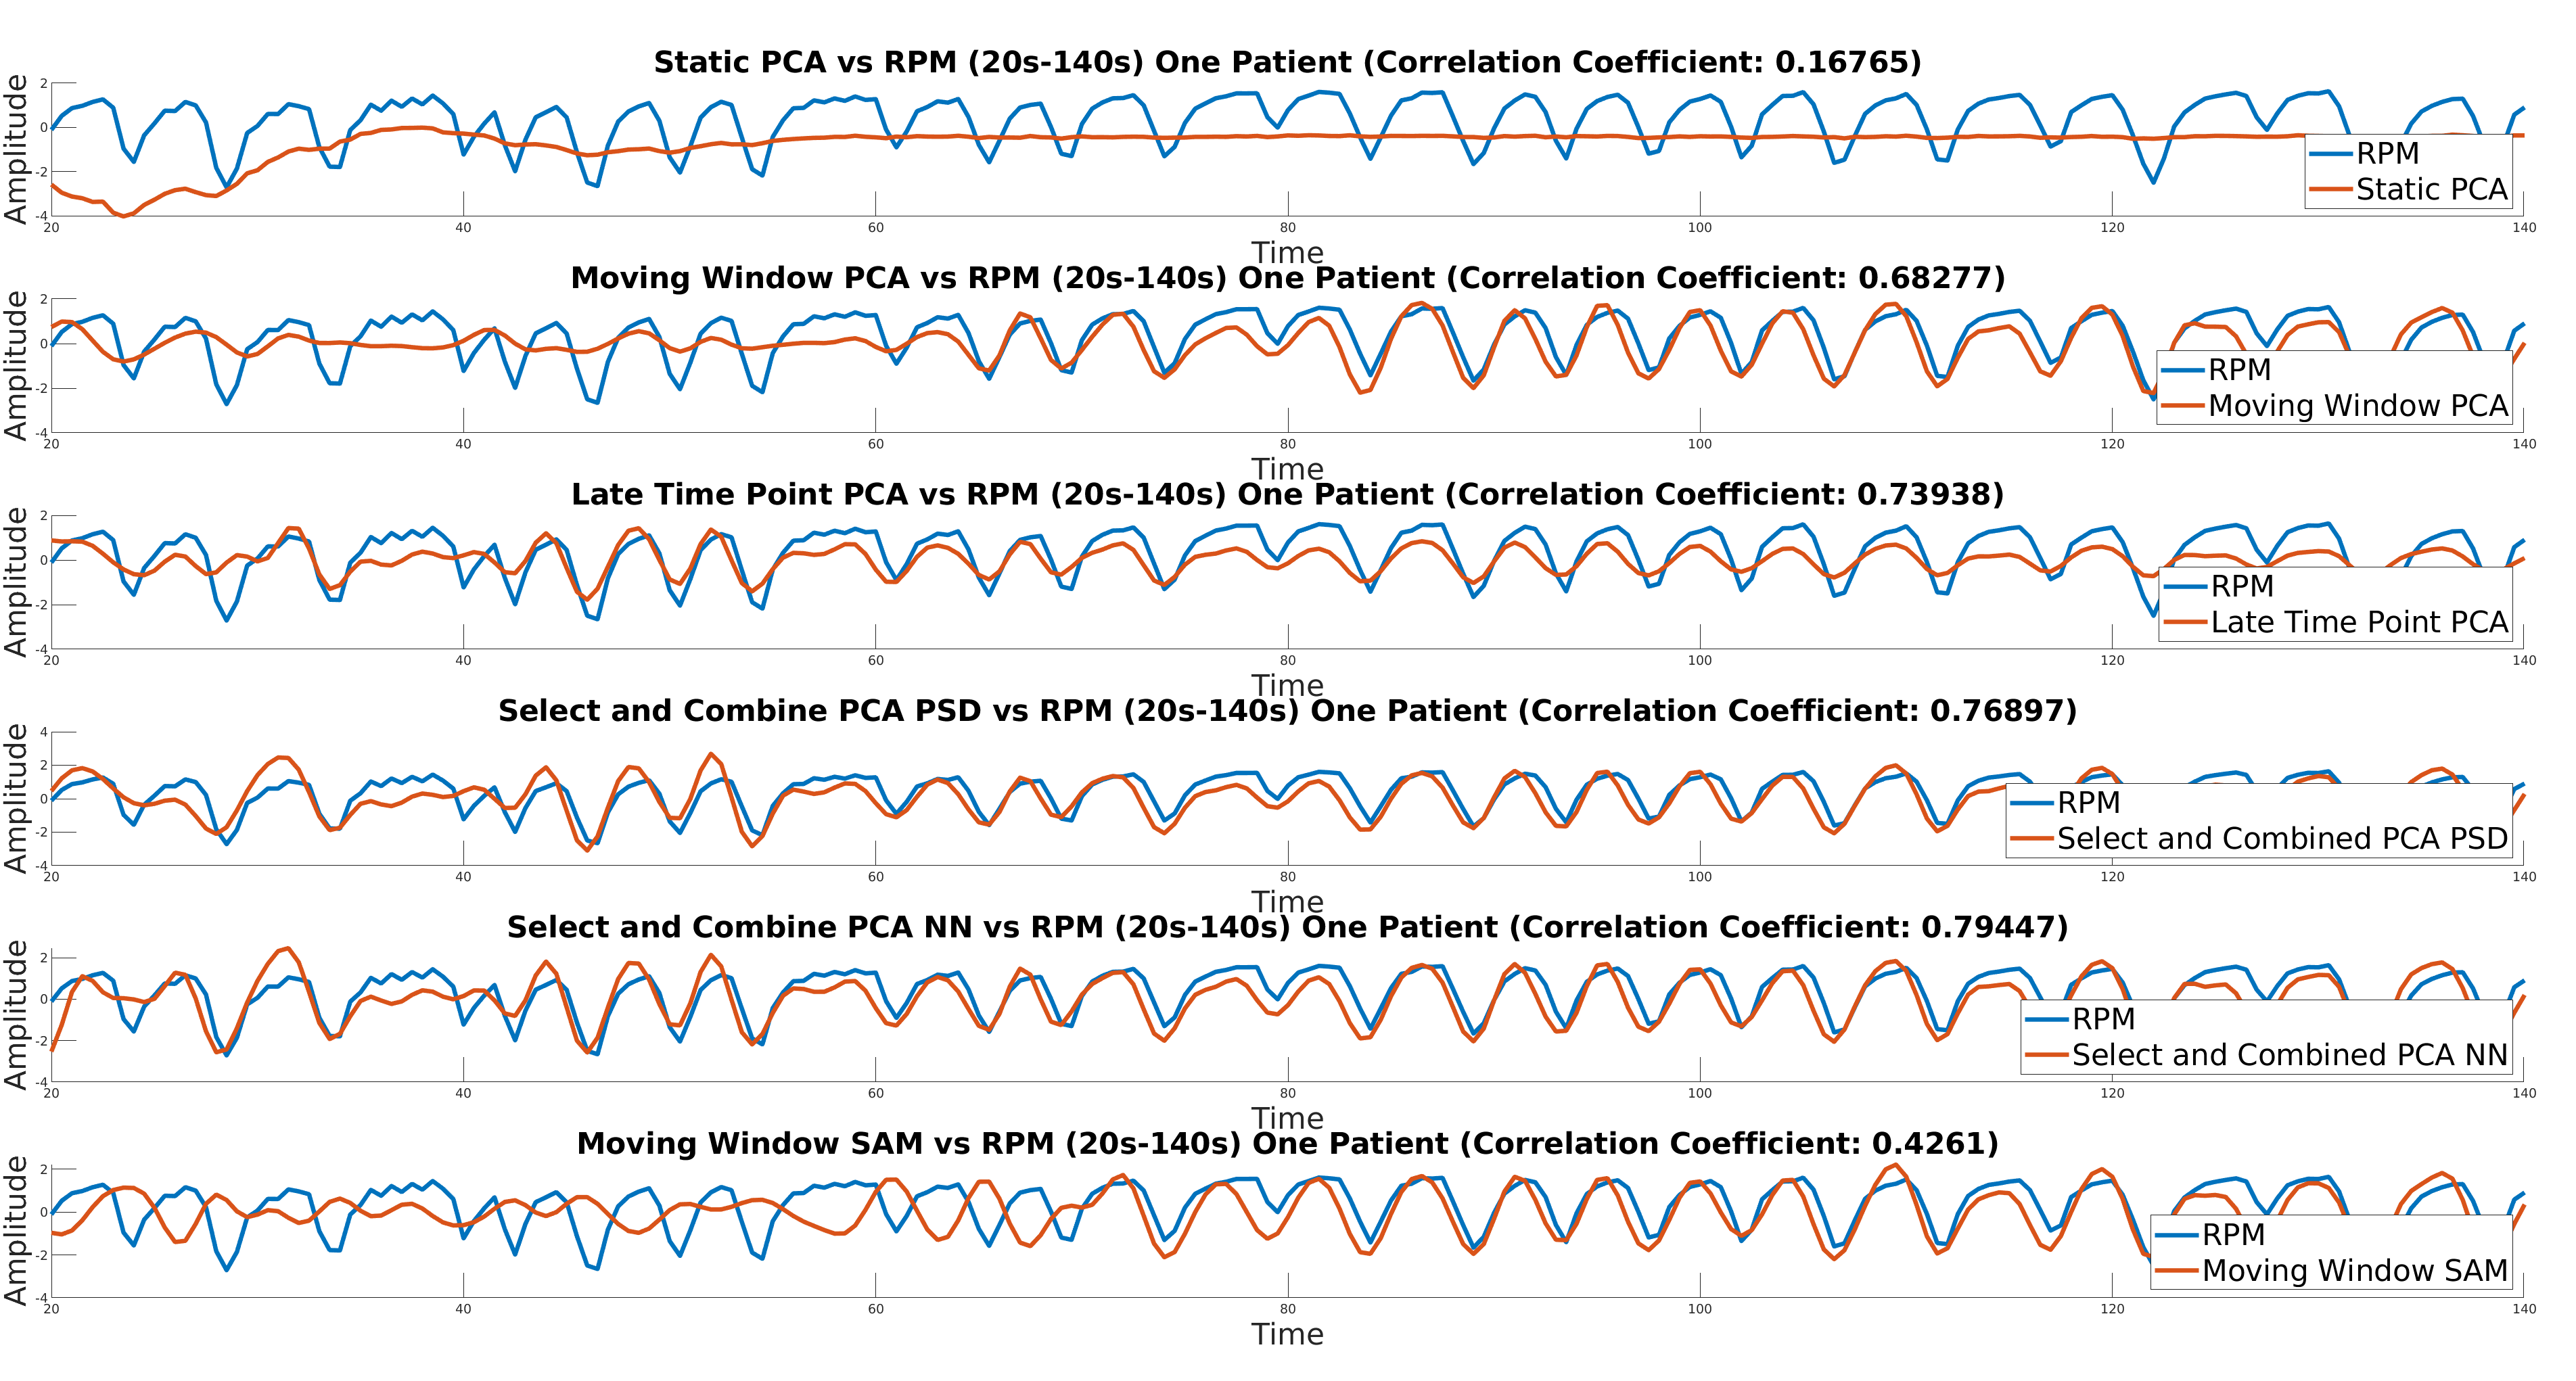
\includegraphics[width=1.0\linewidth]{figures/patient_one_output.png}
        
        \captionsetup{singlelinecheck=false, justification=centering}
        \caption{A plot showing for each method its output compared to the \gls{RPM} for the first \SI{120}{\second} (between \SI{20}{\second} and \SI{140}{\second}) (taken for the first acquisition of patient one). This is for static \gls{PCA}, Moving Window \gls{PCA}, Late Time Frame \gls{PC}, Select and Combine, Select and Combine using a Neural Network and the moving window \gls{SAM} method.}
        \label{fig:patient_one_output}
    \end{figure}
    
    \begin{figure}
        \centering
        
        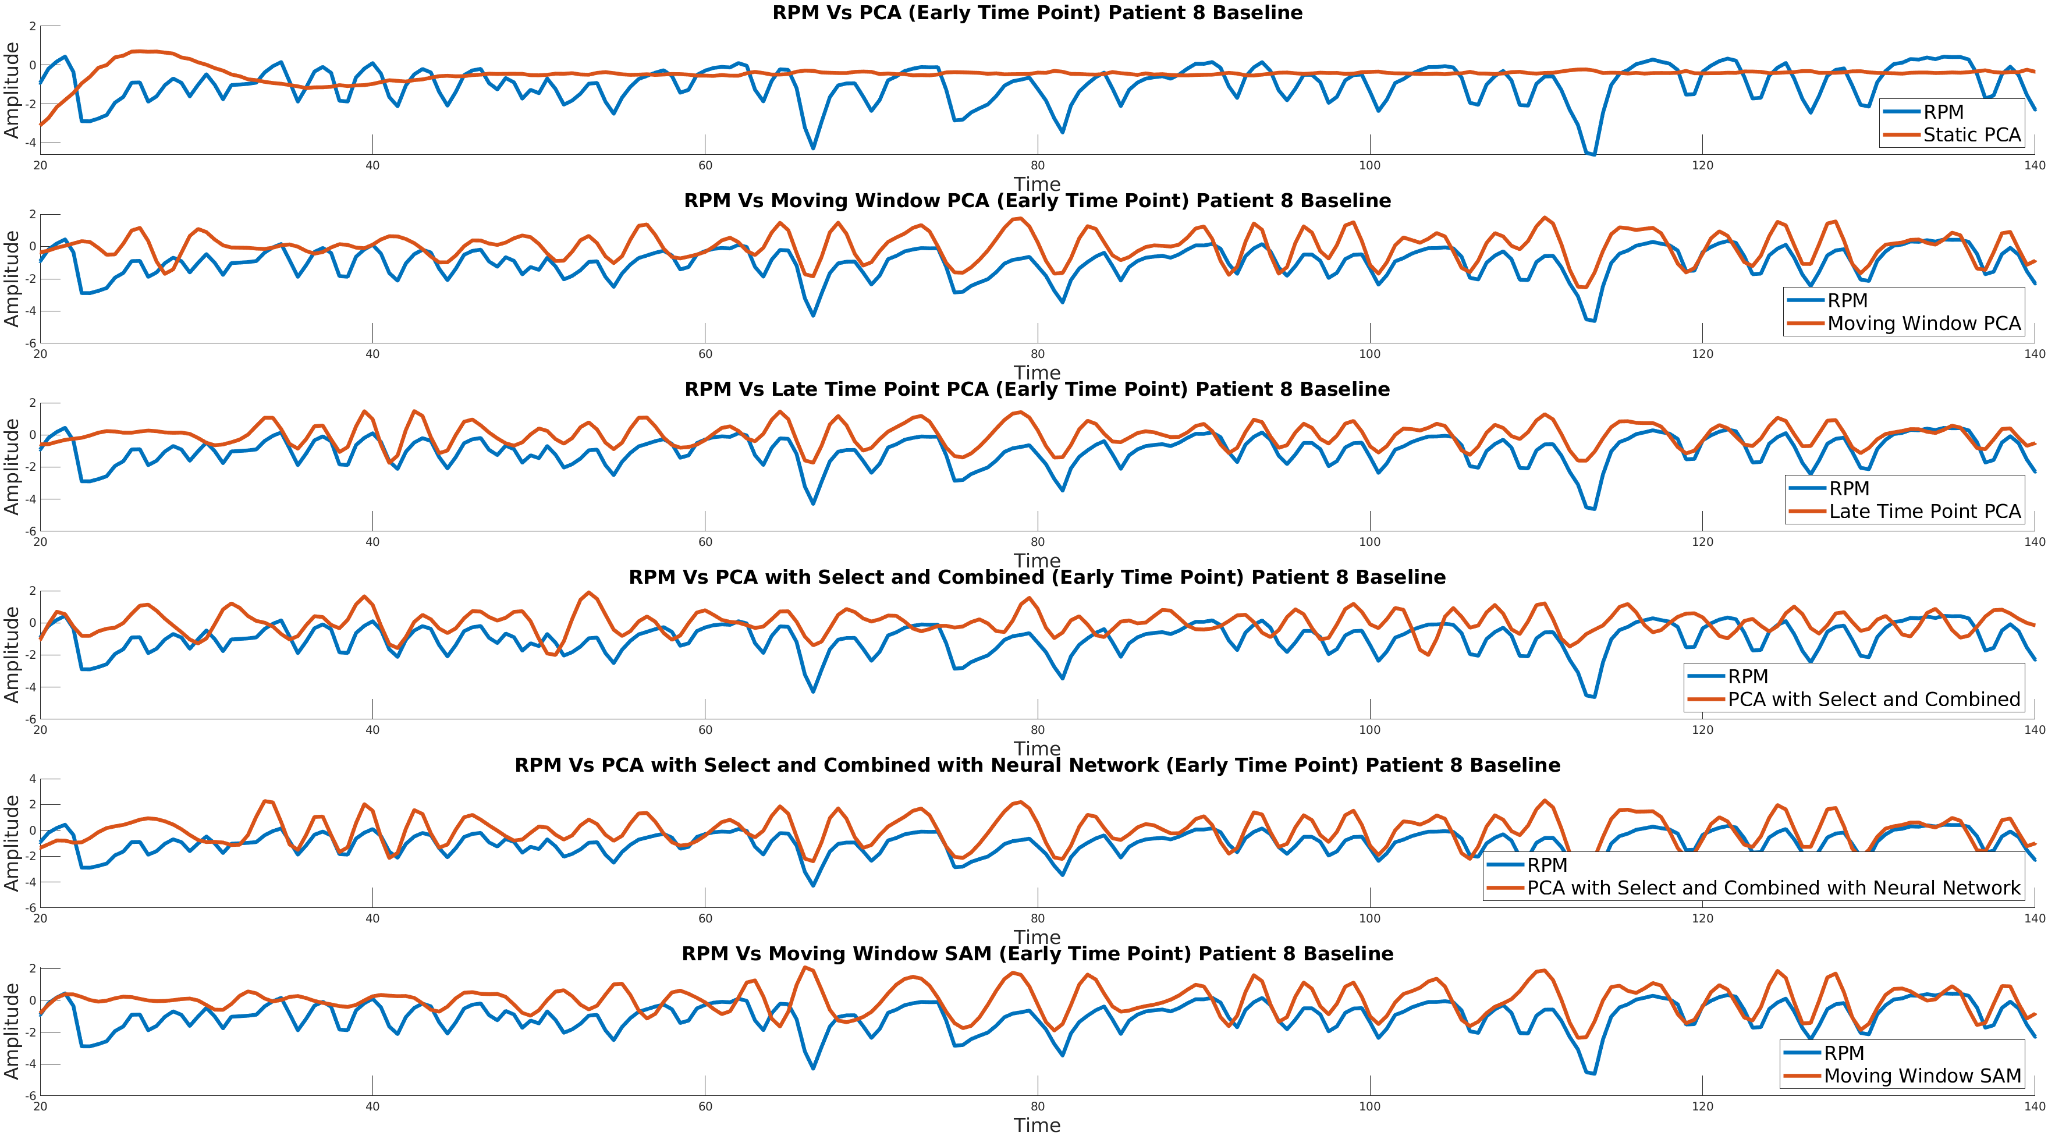
\includegraphics[width=1.0\linewidth]{figures/patient_eight_output.png}
        
        \captionsetup{singlelinecheck=false, justification=centering}
        \caption{A plot showing for each method its output compared to the \gls{RPM} for the first \SI{120}{\second} (between \SI{20}{\second} and \SI{140}{\second}) (taken for the first acquisition of patient eight). This is for static \gls{PCA}, Moving Window \gls{PCA}, Late Time Frame \gls{PC}, Select and Combine, Select and Combine using a Neural Network and the moving window \gls{SAM} method.}
        \label{fig:patient_eight_output}
    \end{figure}
    
    \begin{figure}
        \centering
        
        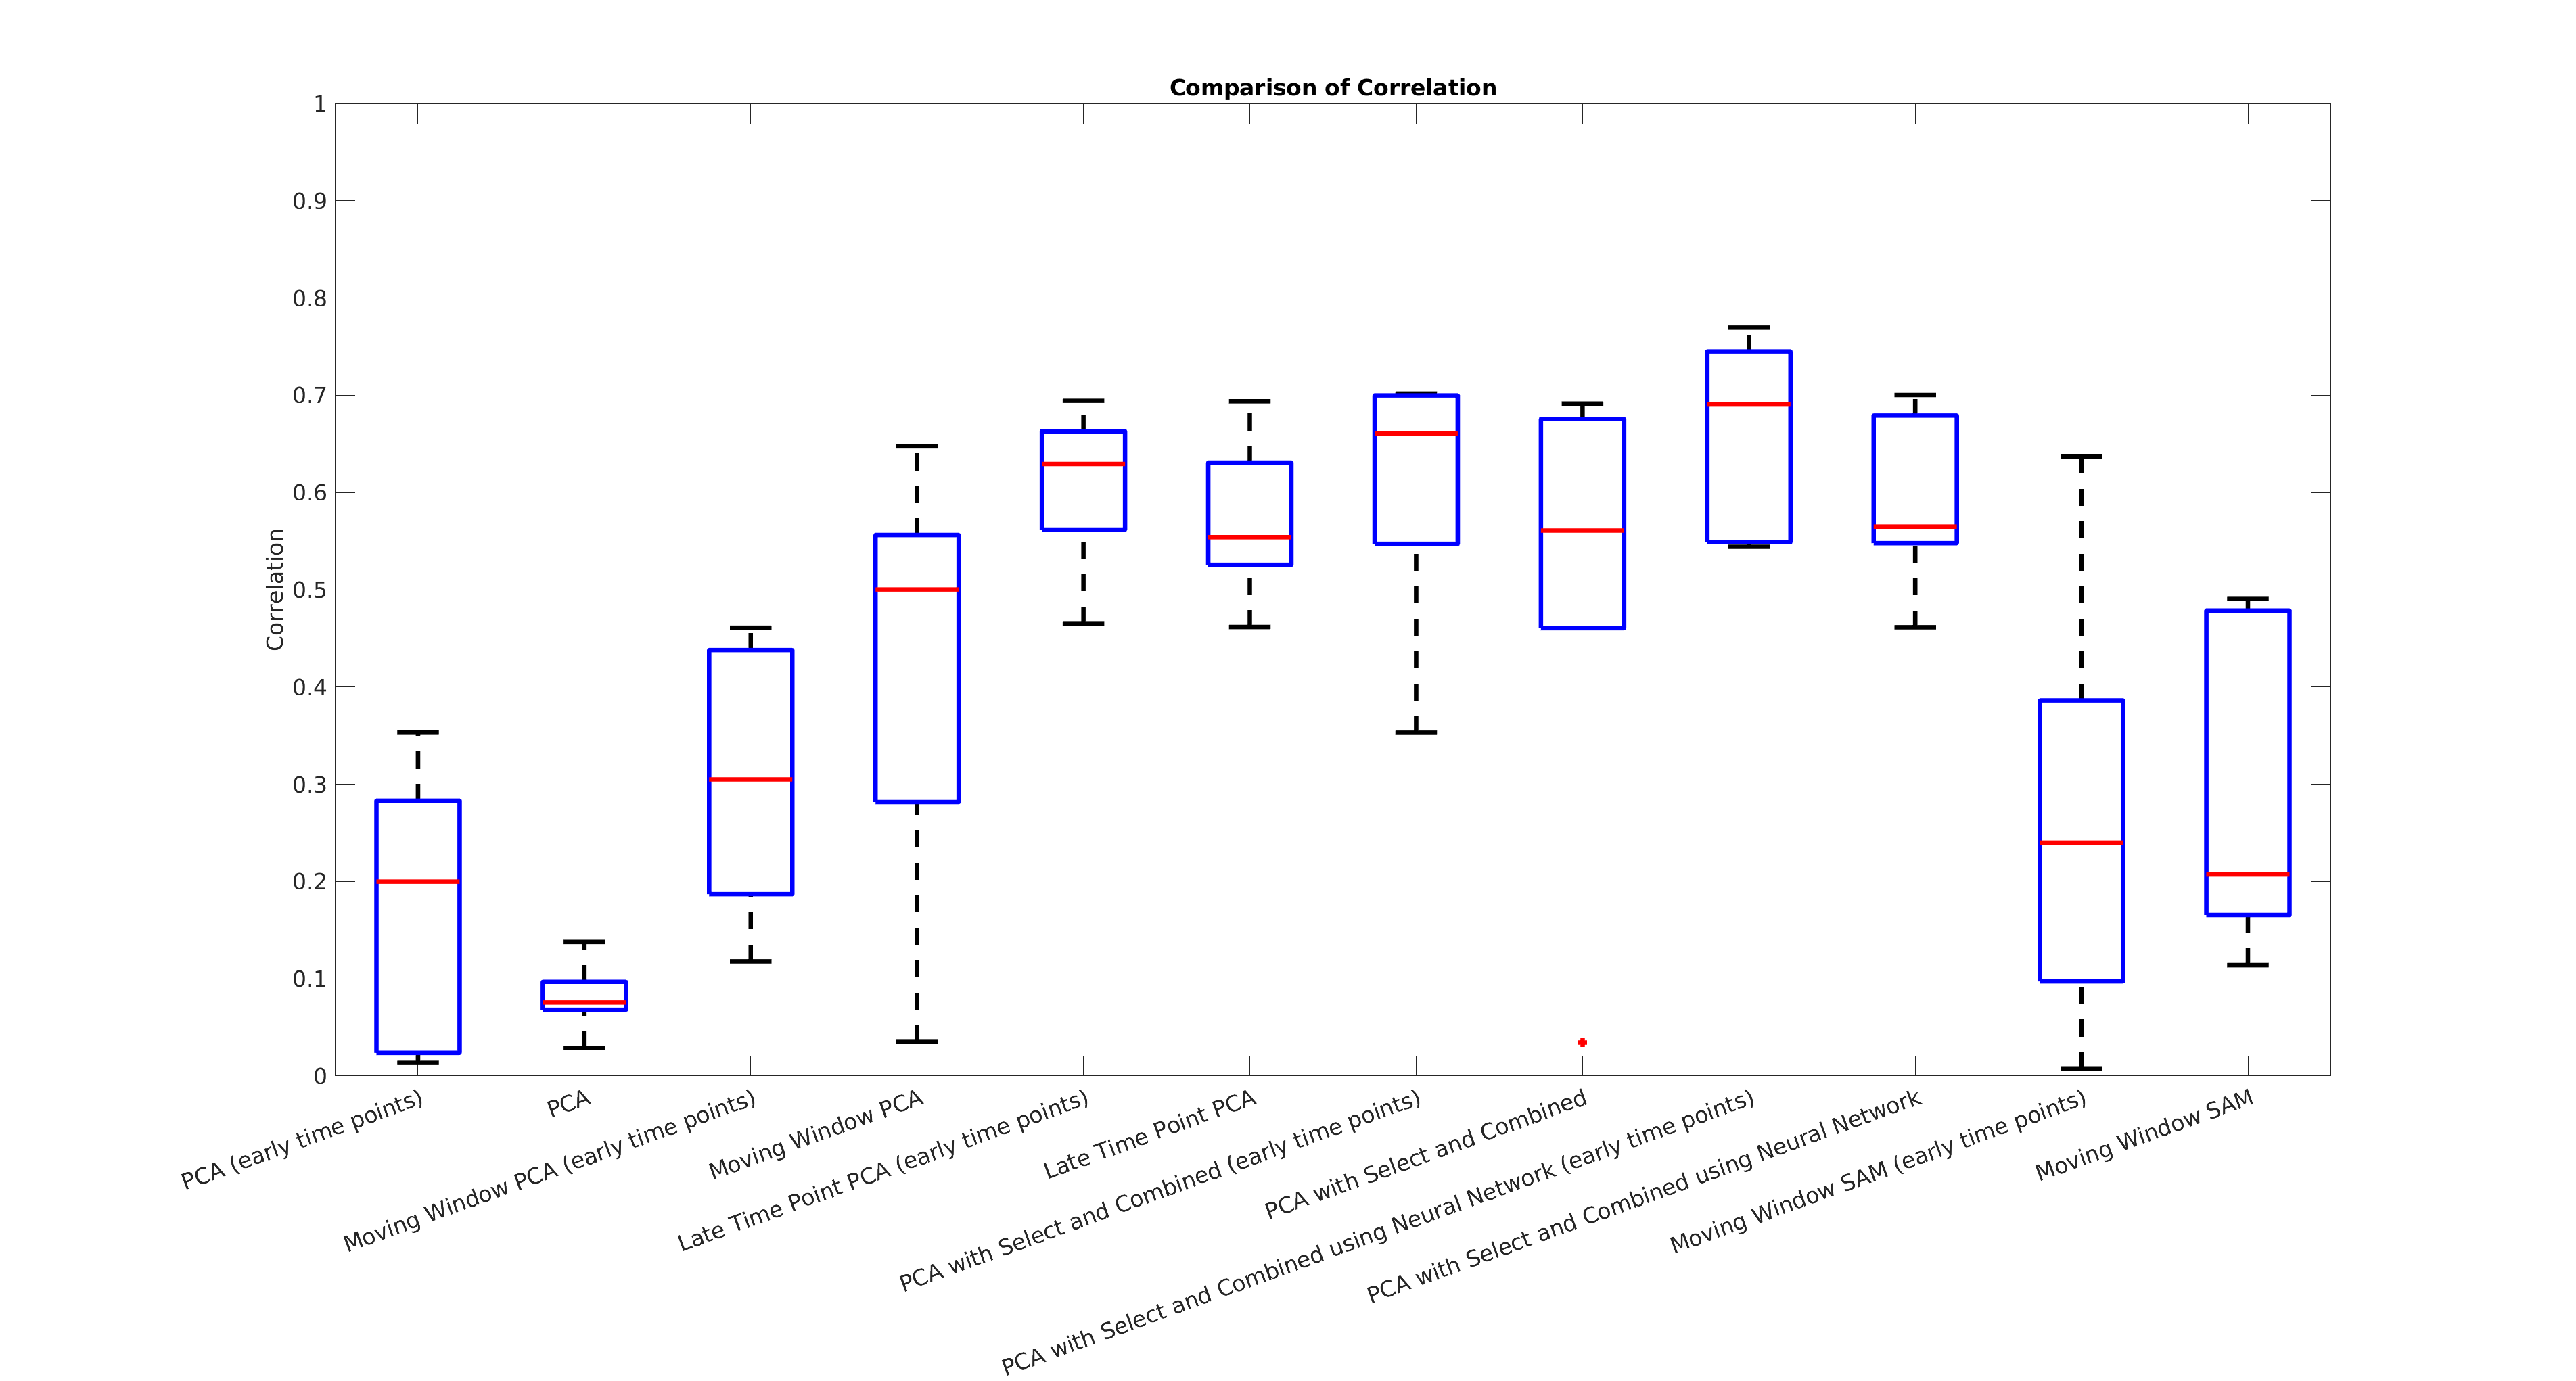
\includegraphics[width=1.0\linewidth]{figures/box_plot.png}
        
        \captionsetup{singlelinecheck=false, justification=centering}
        \caption{A box plot showing for each method its correlation coefficient to the \gls{RPM} for both the first \SI{120}{\second} (between \SI{20}{\second} and \SI{140}{\second}) and also for the entire acquisition (taken for seven acquisitions). This is for static \gls{PCA}, Moving Window \gls{PCA}, Late Time Frame \gls{PC}, Select and Combine, Select and Combine using a Neural Network and the moving window \gls{SAM} method.}
        \label{fig:box_plot}
    \end{figure}
    
        \begin{figure}
        \centering
        
        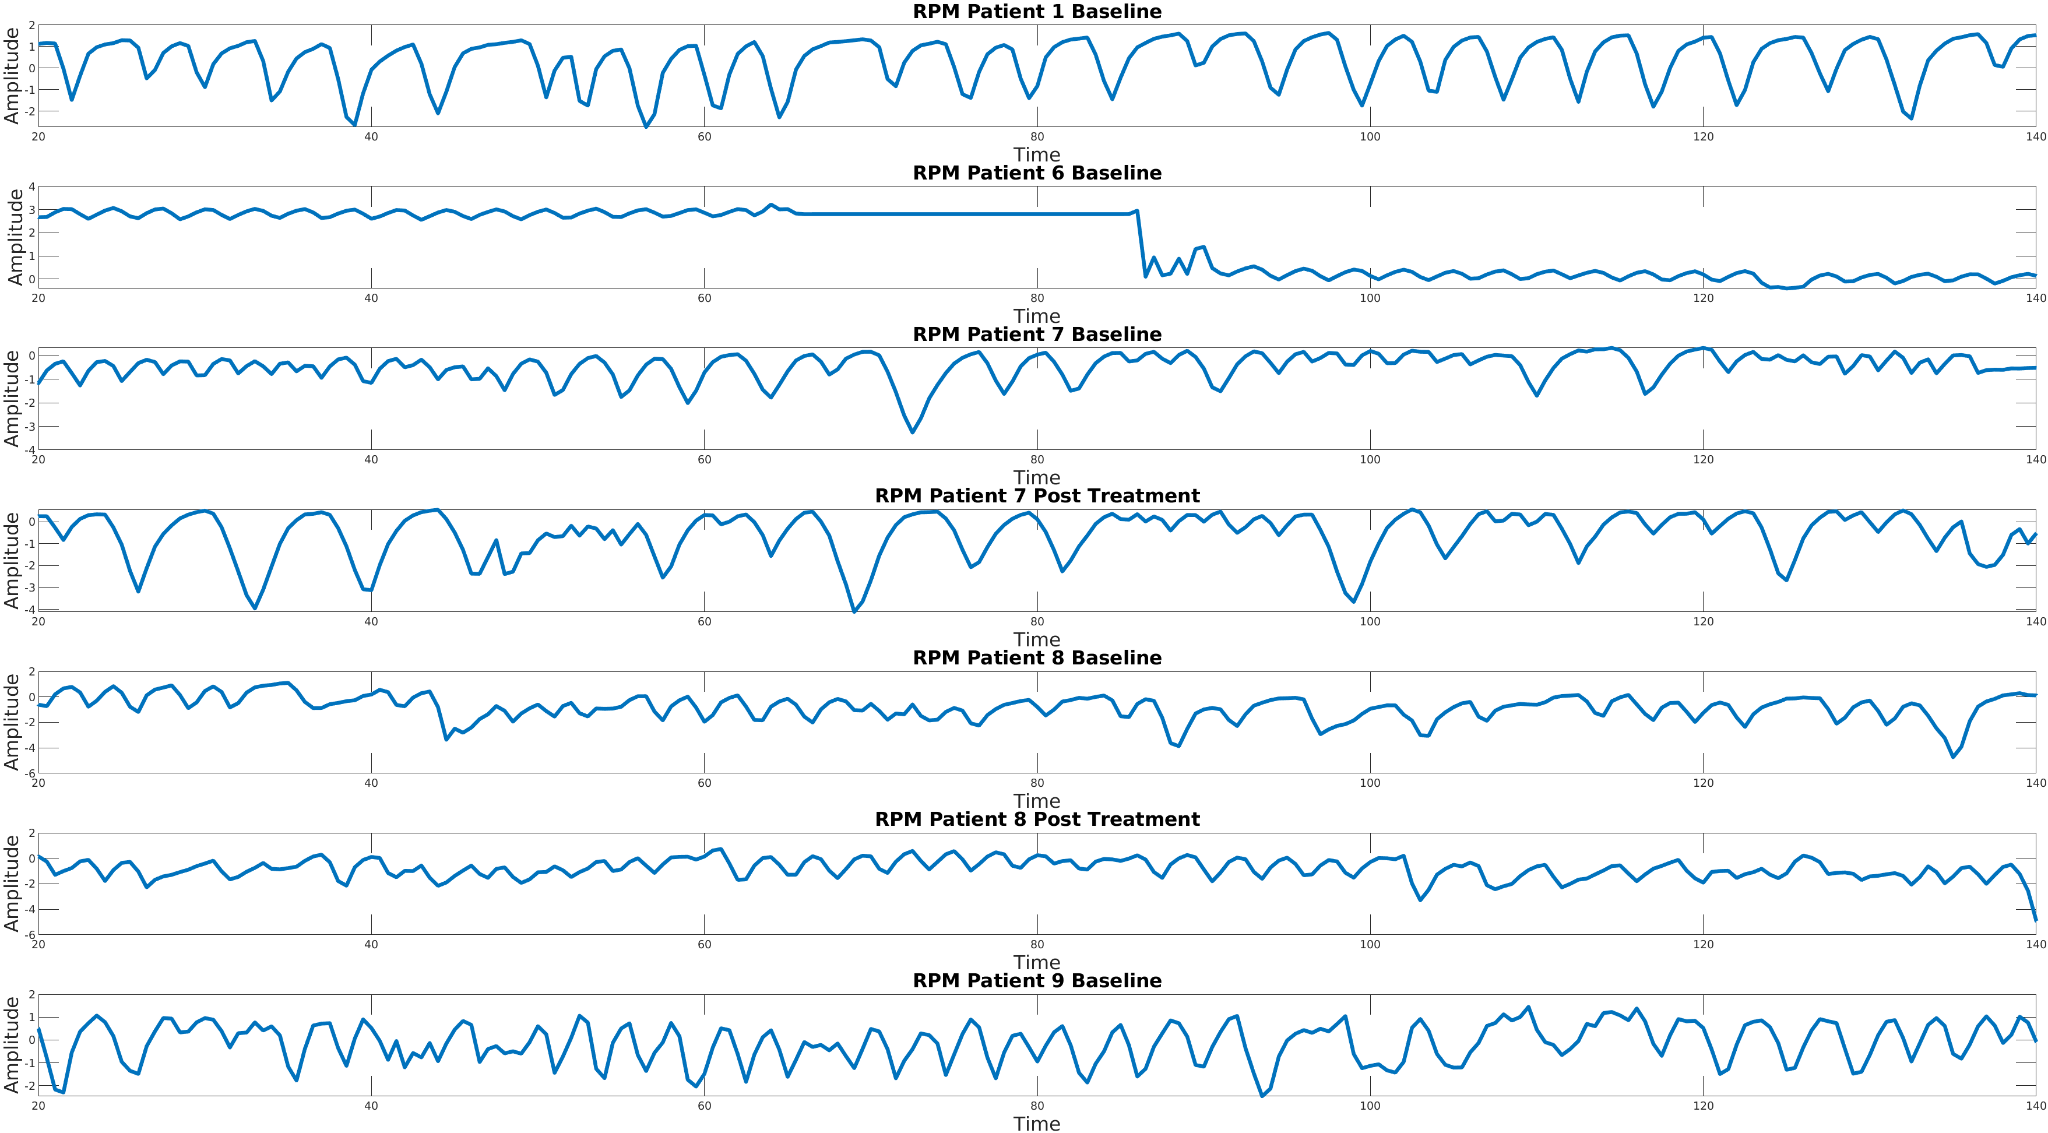
\includegraphics[width=1.0\linewidth]{figures/rpm_signals.png}
        
        \captionsetup{singlelinecheck=false, justification=centering}
        \caption{A plot showing the \gls{RPM} for the first \SI{120}{\second} (between \SI{20}{\second} and \SI{140}{\second}) (taken for seven acquisitions). Notice that only the first acquisition of patient one shows a steady trace with an average frequency, every other trace shows variable breathing or artefacts.}
        \label{fig:rpm_signals}
    \end{figure}
    
    \begin{figure}
        \centering
        
        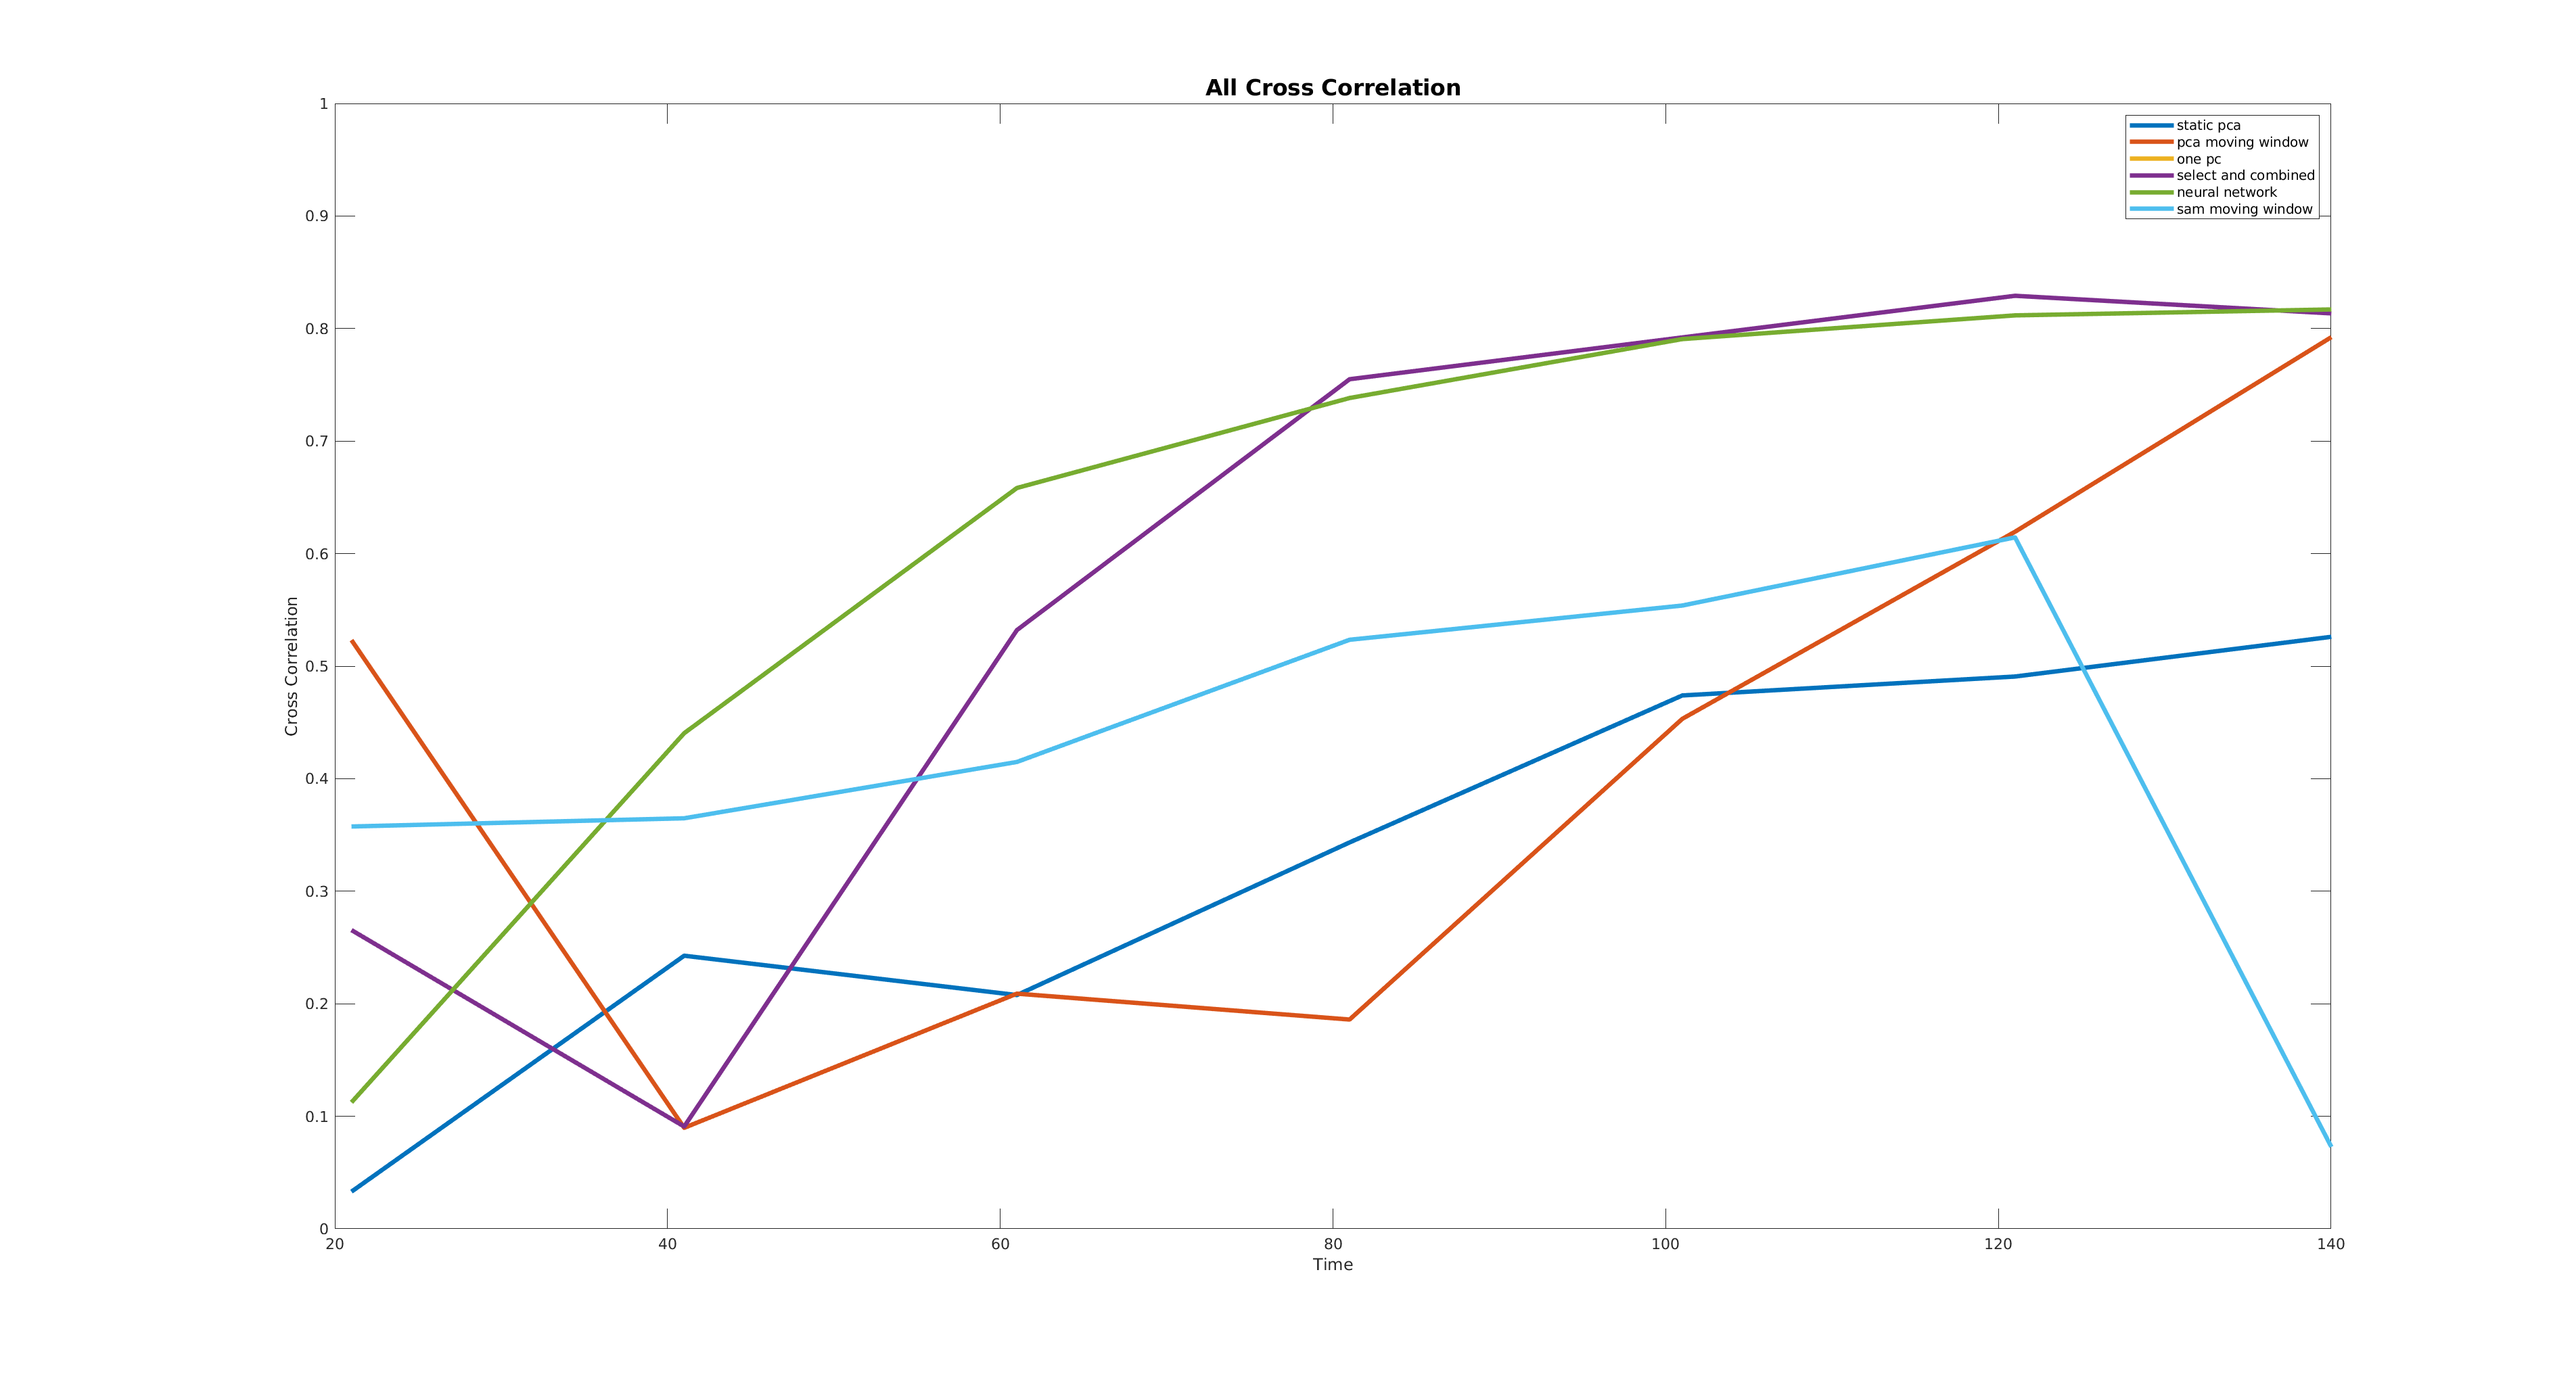
\includegraphics[width=1.0\linewidth]{figures/all_cross_correlation.png}
        
        \captionsetup{singlelinecheck=false, justification=centering}
        \caption{A plot showing for each method its correlation coefficient to the \gls{RPM} for the first \SI{120}{\second} (between \SI{20}{\second} and \SI{140}{\second}) (taken as a mean for all data). This is for static \gls{PCA}, Moving Window \gls{PCA}, Late Time Frame \gls{PC}, Select and Combine, Select and Combine using a Neural Network and the moving window \gls{SAM} method.}
        \label{fig:all_cross_correlation}
    \end{figure}
    
    \begin{figure}
        \centering
        
        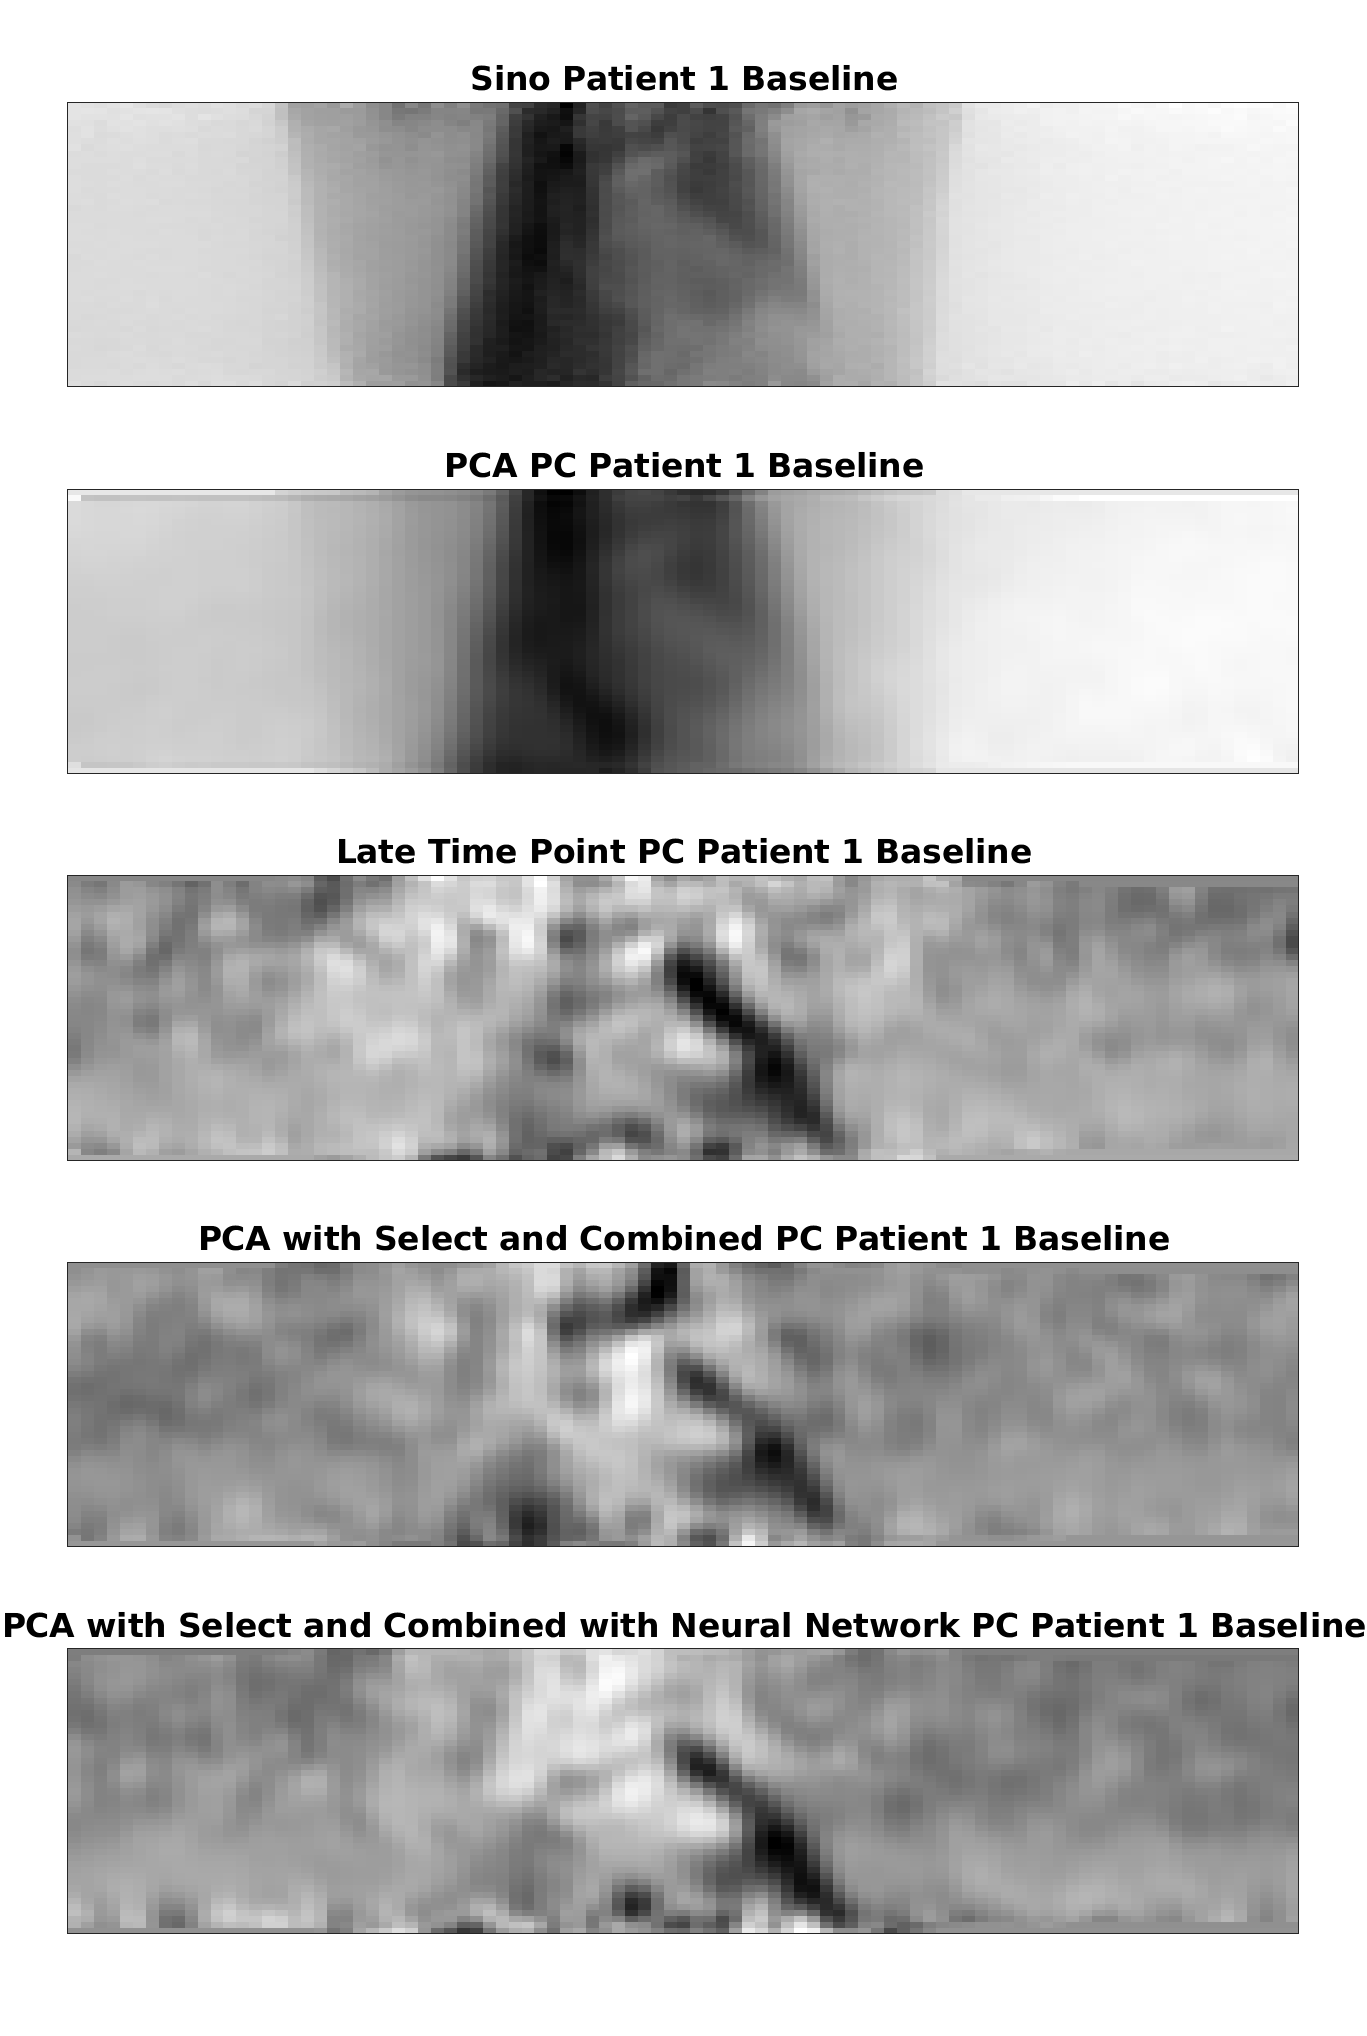
\includegraphics[width=1.0\linewidth]{figures/patient_one_pc_output.png}
        
        \captionsetup{singlelinecheck=false, justification=centering}
        \caption{A plot showing the \gls{PC} used to generate the output signal (taken for the first acquisition of patient eight).}
        \label{fig:patient_one_pc_output}
    \end{figure}
    
    A plot showing for each method its output compared to the \gls{RPM} for the first \SI{120}{\second} (between \SI{20}{\second} and \SI{140}{\second}) (taken for the first acquisition of patient one). This is for static \gls{PCA}, Moving Window \gls{PCA}, Late Time Frame \gls{PC}, Select and Combine, Select and Combine using a Neural Network and the moving window \gls{SAM} method can be seen in~\Fref{fig:patient_one_output}. From a visual analysis it can be observed that the static \gls{PCA} method has failed, post normalisation it appears almost as if there is no variation in the signal at early time points. Both moving window methods show towards the end of the plot that they can extract a signal, however it takes till between \SI{60}{\second} and \SI{80}{\second} until both methods begin to pickup the signal. For the \gls{SAM} based method it appears as if the sign determination method has failed before \SI{80}{\second}, regardless though the method still cannot extract a signal before \SI{60}{\second}. The Late Time Frame \gls{PC}, Select and Combine and Select and Combine using a Neural Network methods all appear to be able to extract a usable signal right down to \SI{20}{\second} (around when counts begin to appear in the \gls{FOV}). The magnitude of the signal post \SI{80}{\second} more closely matches the \gls{RPM} (or in comparison to before \SI{80}{\second}) for both Select and Combine methods than for the Late Time Frame \gls{PC} method.
    
    A plot showing for each method its output compared to the \gls{RPM} for the first \SI{120}{\second} (between \SI{20}{\second} and \SI{140}{\second}) (taken for the first acquisition of patient eight). This is for static \gls{PCA}, Moving Window \gls{PCA}, Late Time Frame \gls{PC}, Select and Combine, Select and Combine using a Neural Network and the moving window \gls{SAM} method can be seen in~\Fref{fig:patient_eight_output}. The same story as for in~\Fref{fig:patient_one_output} seems to hold here, although all methods match the \gls{RPM} worse than in~\Fref{fig:patient_one_output}. This acquisition was selected to be shown due to it being a difficult trace to extract. Regardless, the Late Time Frame \gls{PC} and Select and Combine methods appear to have extracted a signal early into the acquisition.
    
    A box plot showing for each method its correlation coefficient to the \gls{RPM} for both the first \SI{120}{\second} (between \SI{20}{\second} and \SI{140}{\second}) and also for the entire acquisition (taken for seven acquisitions). This is for static \gls{PCA}, Moving Window \gls{PCA}, Late Time Frame \gls{PC}, Select and Combine, Select and Combine using a Neural Network and the moving window \gls{SAM} method can be seen in~\Fref{fig:box_plot}. Here the improvement of the Late Time Frame \gls{PC} and by incorporating multiple \glss{PC} is most apparent. The correlation coefficient for the static \gls{PCA} method is as would be expected, the correlation coefficient is low and as such the method is not usable. The correlation coefficient for both the moving window methods are similar, thus proving the hypothesis stated above in~\Fref{sec:moving_window} is plausible regardless of the method used to extract the signal for each window. However, again here the correlation coefficient is lower than is acceptable, the discrepancy here between the results shown in~\cite{Schleyer2014} could be attributed to the complexity of the data (this is shown in~\Fref{fig:rpm_signals}). Continuing, the results from the Late Time Frame \gls{PC}, Select and Combine and Select and Combine using a Neural Network methods all show high correlation coefficient for both the early time point as well as for all data. The Select and Combine methods show marginally higher correlation coefficient than the Late Time Frame \gls{PC} method and the neural network shows slightly higher correlation coefficient than the frequency based scoring.
    
    A plot showing for each method its correlation coefficient to the \gls{RPM} for the first \SI{120}{\second} (between \SI{20}{\second} and \SI{140}{\second}) (taken as a mean for all data). This is for static \gls{PCA}, Moving Window \gls{PCA}, Late Time Frame \gls{PC}, Select and Combine, Select and Combine using a Neural Network and the moving window \gls{SAM} method can be seen in~\Fref{fig:all_cross_correlation}. Here it can be observed that on average across all results all methods struggle to produce usable results more often than not at the very beginning of the acquisition (around when counts begin to appear in the \gls{FOV}). However, it is also apparent that on average both Select and Combine methods robustly begin to produce results which closely match the \gls{RPM}, as evidenced by a reasonable correlation past the first \SI{40}{\second} on most acquisitions.
    
    A plot showing the \gls{PC} used to generate the output signal (taken for the first acquisition of patient eight) can be seen in~\Fref{fig:patient_one_pc_output}. Here it can be observed the difference in the \gls{PC} resulting from each method. The static \gls{PCA} method returns a \gls{PC} which closely resembles the input data, leading to the conclusion that variation from a number of sources is included. However, each other method produces a \gls{PC} which can only be differentiated by the level of noise apparent in the \gls{PC}. It appears from a visual inspection that the least confounding variation and noise is included in the Select and Combine with Neural Network method.

% \vspace{-0.3cm}
    
\section{Discussion} \label{sec:discussion}
    The work presented here suffers from a few limitations. Firstly, the data used here all originates from the same study, using the same procedure, the same radiotracer and acquired on the same scanner. In order to better validate the generalisability of the method it would be positive to test on data acquired on different scanners and using different radiotracers. Additionally, from the data acquired only a subset of this data is usable due to issues during acquisition, the number of participants is limited. It would be beneficial to test the methods on a larger sample of patients, with both a larger number of non-complex and complex breathers to better test the limitations of the methods.
    
    An additional concern is the point at which the methods may fail for patients who exhibit abnormal breathing patters. For instance, extremely slow breathers will breathe at a rate less than \SI{0.1}{\hertz}, which here would be considered to be radiotracer kinetics in the Select and Combine methods case. Furthermore, the method struggles with patients who breathe at less regular intervals, exemplified by those who occasionally hold their breath or otherwise stop breathing for periods and by those who breathe in such a way as to induce multiple harmonics in their breathing (this could be seen as a signal atop a carrier).

% \vspace{-0.3cm}

\section{Conclusion} \label{sec:conclusion}
    Results from a visual comparison of early time point output signals compared to the \gls{RPM}, quality of \gls{PC} and also when looking at the correlation coefficient of the output signals to the \gls{RPM} indicates that the Late Time Frame \gls{PC} and both Select and Combine methods are more robust and afford higher quality signals than both moving window methods. The results also indicate that both Select and Combine methods can give a higher correlation coefficient earlier than the Late Time Frame \gls{PC} method and that the neural network shows slightly higher correlation coefficient than the frequency based scoring. The selection of which method to use would be down to the goals of those implementing them and the available tools.
    
    In the future, research will focus on further development of the method, including optimisation of the neural network scoring method. In the next stage, these methods will be applied to the task of implementing advanced respiratory motion correction on dynamic \gls{PET} data.